% Created by tikzDevice version 0.12 on 2019-04-11 07:16:34
% !TEX encoding = UTF-8 Unicode
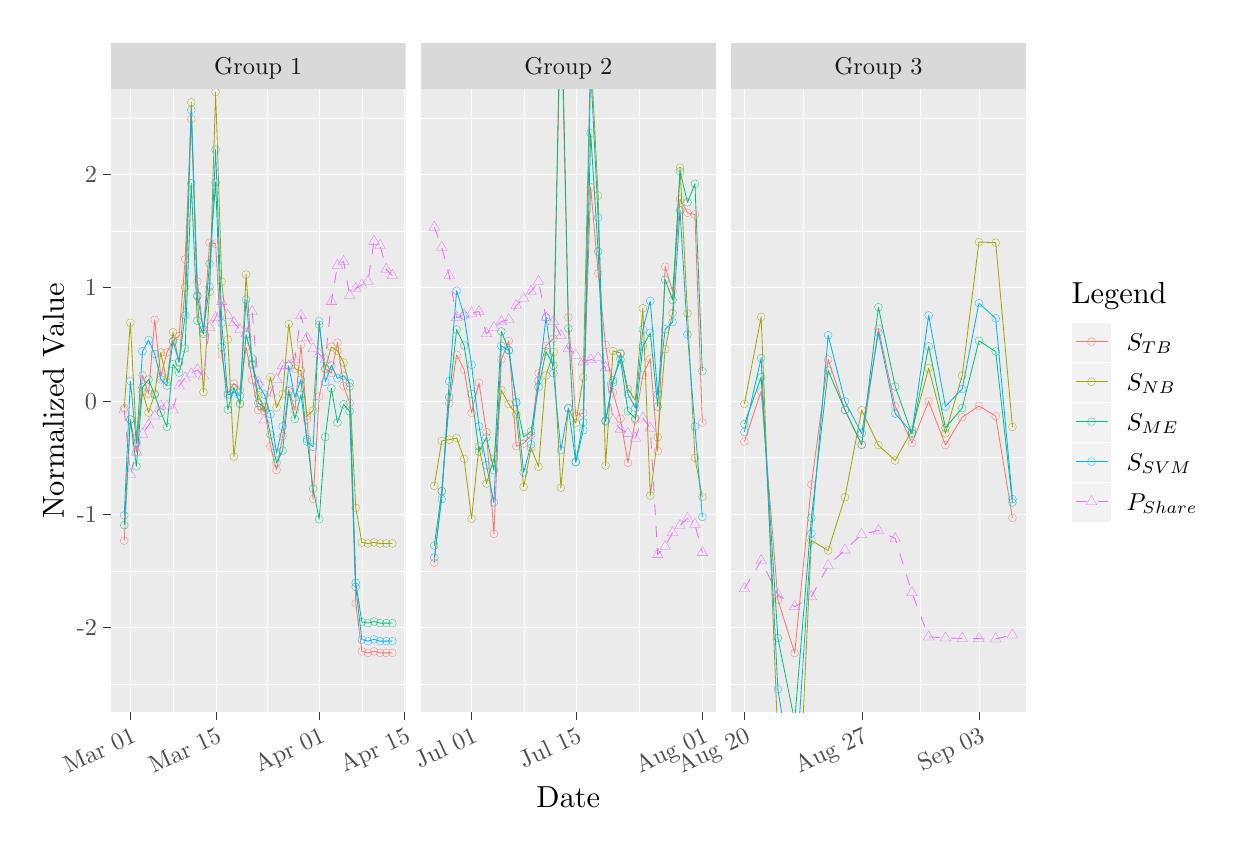
\begin{tikzpicture}[x=1pt,y=1pt]
\definecolor{fillColor}{RGB}{255,255,255}
\path[use as bounding box,fill=fillColor,fill opacity=0.00] (0,0) rectangle (433.62,289.08);
\begin{scope}
\path[clip] (  0.00,  0.00) rectangle (433.62,289.08);
\definecolor{drawColor}{RGB}{255,255,255}
\definecolor{fillColor}{RGB}{255,255,255}

\path[draw=drawColor,line width= 0.1pt,line join=round,line cap=round,fill=fillColor] (  0.00,  0.00) rectangle (433.62,289.08);
\end{scope}
\begin{scope}
\path[clip] ( 30.06, 41.66) rectangle (136.60,266.77);
\definecolor{fillColor}{gray}{0.92}

\path[fill=fillColor] ( 30.06, 41.66) rectangle (136.60,266.77);
\definecolor{drawColor}{RGB}{255,255,255}

\path[draw=drawColor,line width= 0.1pt,line join=round] ( 30.06, 51.89) --
	(136.60, 51.89);

\path[draw=drawColor,line width= 0.1pt,line join=round] ( 30.06, 92.82) --
	(136.60, 92.82);

\path[draw=drawColor,line width= 0.1pt,line join=round] ( 30.06,133.75) --
	(136.60,133.75);

\path[draw=drawColor,line width= 0.1pt,line join=round] ( 30.06,174.68) --
	(136.60,174.68);

\path[draw=drawColor,line width= 0.1pt,line join=round] ( 30.06,215.61) --
	(136.60,215.61);

\path[draw=drawColor,line width= 0.1pt,line join=round] ( 30.06,256.54) --
	(136.60,256.54);

\path[draw=drawColor,line width= 0.1pt,line join=round] ( 52.51, 41.66) --
	( 52.51,266.77);

\path[draw=drawColor,line width= 0.1pt,line join=round] ( 86.63, 41.66) --
	( 86.63,266.77);

\path[draw=drawColor,line width= 0.1pt,line join=round] (120.75, 41.66) --
	(120.75,266.77);

\path[draw=drawColor,line width= 0.1pt,line join=round] ( 30.06, 72.36) --
	(136.60, 72.36);

\path[draw=drawColor,line width= 0.1pt,line join=round] ( 30.06,113.29) --
	(136.60,113.29);

\path[draw=drawColor,line width= 0.1pt,line join=round] ( 30.06,154.22) --
	(136.60,154.22);

\path[draw=drawColor,line width= 0.1pt,line join=round] ( 30.06,195.15) --
	(136.60,195.15);

\path[draw=drawColor,line width= 0.1pt,line join=round] ( 30.06,236.08) --
	(136.60,236.08);

\path[draw=drawColor,line width= 0.1pt,line join=round] ( 37.10, 41.66) --
	( 37.10,266.77);

\path[draw=drawColor,line width= 0.1pt,line join=round] ( 67.92, 41.66) --
	( 67.92,266.77);

\path[draw=drawColor,line width= 0.1pt,line join=round] (105.34, 41.66) --
	(105.34,266.77);

\path[draw=drawColor,line width= 0.1pt,line join=round] (136.16, 41.66) --
	(136.16,266.77);
\definecolor{drawColor}{RGB}{248,118,109}

\path[draw=drawColor,line width= 0.3pt,line join=round] ( 34.90,103.73) --
	( 37.10,147.53) --
	( 39.30,135.75) --
	( 41.50,163.46) --
	( 43.70,156.80) --
	( 45.90,183.50) --
	( 48.11,163.02) --
	( 50.31,171.72) --
	( 52.51,175.98) --
	( 54.71,177.63) --
	( 56.91,205.36) --
	( 59.11,256.05) --
	( 61.31,197.33) --
	( 63.52,178.99) --
	( 65.72,211.38) --
	( 67.92,211.02) --
	( 70.12,170.93) --
	( 72.32,156.86) --
	( 74.52,160.46) --
	( 76.72,158.17) --
	( 78.92,173.72) --
	( 81.13,161.79) --
	( 83.33,150.90) --
	( 85.53,151.73) --
	( 87.73,137.79) --
	( 89.93,129.24) --
	( 92.13,141.44) --
	( 94.33,158.29) --
	( 96.53,150.83) --
	( 98.74,174.44) --
	(100.94,147.39) --
	(103.14,118.78) --
	(105.34,155.82) --
	(107.54,165.91) --
	(109.74,164.24) --
	(111.94,175.30) --
	(114.15,159.62) --
	(116.35,153.50) --
	(118.55, 81.05) --
	(120.75, 63.71) --
	(122.95, 63.16) --
	(125.15, 63.71) --
	(127.35, 63.16) --
	(129.55, 63.16) --
	(131.76, 63.17);
\definecolor{drawColor}{RGB}{163,165,0}

\path[draw=drawColor,line width= 0.3pt,line join=round] ( 34.90,151.59) --
	( 37.10,182.46) --
	( 39.30,141.04) --
	( 41.50,157.50) --
	( 43.70,150.00) --
	( 45.90,156.87) --
	( 48.11,171.74) --
	( 50.31,160.98) --
	( 52.51,179.04) --
	( 54.71,168.01) --
	( 56.91,195.32) --
	( 59.11,262.09) --
	( 61.31,191.95) --
	( 63.52,157.40) --
	( 65.72,193.58) --
	( 67.92,265.80) --
	( 70.12,197.33) --
	( 72.32,176.39) --
	( 74.52,134.07) --
	( 76.72,153.30) --
	( 78.92,199.87) --
	( 81.13,167.59) --
	( 83.33,156.30) --
	( 85.53,150.55) --
	( 87.73,162.90) --
	( 89.93,151.81) --
	( 92.13,156.67) --
	( 94.33,181.95) --
	( 96.53,165.89) --
	( 98.74,165.16) --
	(100.94,148.75) --
	(103.14,150.78) --
	(105.34,181.74) --
	(107.54,165.69) --
	(109.74,173.78) --
	(111.94,172.30) --
	(114.15,168.08) --
	(116.35,159.37) --
	(118.55,115.56) --
	(120.75,103.07) --
	(122.95,102.67) --
	(125.15,103.09) --
	(127.35,102.70) --
	(129.55,102.69) --
	(131.76,102.71);
\definecolor{drawColor}{RGB}{0,191,125}

\path[draw=drawColor,line width= 0.3pt,line join=round] ( 34.90,109.30) --
	( 37.10,147.44) --
	( 39.30,130.57) --
	( 41.50,159.08) --
	( 43.70,161.92) --
	( 45.90,156.40) --
	( 48.11,150.01) --
	( 50.31,144.85) --
	( 52.51,167.44) --
	( 54.71,164.43) --
	( 56.91,173.19) --
	( 59.11,232.82) --
	( 61.31,183.16) --
	( 63.52,178.38) --
	( 65.72,203.79) --
	( 67.92,233.17) --
	( 70.12,173.73) --
	( 72.32,151.08) --
	( 74.52,158.97) --
	( 76.72,153.10) --
	( 78.92,178.18) --
	( 81.13,169.58) --
	( 83.33,153.43) --
	( 85.53,152.07) --
	( 87.73,142.04) --
	( 89.93,131.88) --
	( 92.13,136.23) --
	( 94.33,157.69) --
	( 96.53,147.69) --
	( 98.74,156.42) --
	(100.94,140.41) --
	(103.14,122.46) --
	(105.34,111.43) --
	(107.54,141.14) --
	(109.74,158.77) --
	(111.94,146.40) --
	(114.15,152.99) --
	(116.35,150.42) --
	(118.55, 88.52) --
	(120.75, 74.34) --
	(122.95, 73.93) --
	(125.15, 74.47) --
	(127.35, 73.92) --
	(129.55, 73.92) --
	(131.76, 73.93);
\definecolor{drawColor}{RGB}{0,176,246}

\path[draw=drawColor,line width= 0.3pt,line join=round] ( 34.90,112.84) --
	( 37.10,161.42) --
	( 39.30,138.93) --
	( 41.50,172.15) --
	( 43.70,176.20) --
	( 45.90,171.15) --
	( 48.11,162.00) --
	( 50.31,159.76) --
	( 52.51,175.69) --
	( 54.71,168.39) --
	( 56.91,185.12) --
	( 59.11,259.33) --
	( 61.31,192.29) --
	( 63.52,180.01) --
	( 65.72,195.46) --
	( 67.92,245.03) --
	( 70.12,182.32) --
	( 72.32,156.33) --
	( 74.52,157.33) --
	( 76.72,156.04) --
	( 78.92,190.81) --
	( 81.13,167.11) --
	( 83.33,160.12) --
	( 85.53,156.50) --
	( 87.73,149.42) --
	( 89.93,135.37) --
	( 92.13,145.03) --
	( 94.33,166.91) --
	( 96.53,155.49) --
	( 98.74,161.89) --
	(100.94,139.54) --
	(103.14,137.62) --
	(105.34,183.06) --
	(107.54,161.07) --
	(109.74,166.99) --
	(111.94,162.35) --
	(114.15,163.31) --
	(116.35,160.68) --
	(118.55, 86.98) --
	(120.75, 67.97) --
	(122.95, 67.41) --
	(125.15, 68.04) --
	(127.35, 67.40) --
	(129.55, 67.40) --
	(131.76, 67.40);
\definecolor{drawColor}{RGB}{231,107,243}

\path[draw=drawColor,line width= 0.3pt,dash pattern=on 4pt off 4pt ,line join=round] ( 34.90,150.93) --
	( 37.10,127.71) --
	( 39.30,135.69) --
	( 41.50,142.22) --
	( 43.70,145.49) --
	( 45.90,148.75) --
	( 48.11,152.38) --
	( 50.31,152.38) --
	( 52.51,150.93) --
	( 54.71,159.64) --
	( 56.91,162.54) --
	( 59.11,163.99) --
	( 61.31,165.44) --
	( 63.52,163.26) --
	( 65.72,180.68) --
	( 67.92,184.31) --
	( 70.12,190.11) --
	( 72.32,185.03) --
	( 74.52,182.49) --
	( 76.72,179.95) --
	( 78.92,178.50) --
	( 81.13,186.48) --
	( 83.33,161.09) --
	( 85.53,147.30) --
	( 87.73,157.10) --
	( 89.93,162.00) --
	( 92.13,166.89) --
	( 94.33,166.89) --
	( 96.53,169.07) --
	( 98.74,185.03) --
	(100.94,177.05) --
	(103.14,173.06) --
	(105.34,171.07) --
	(107.54,169.07) --
	(109.74,190.11) --
	(111.94,203.17) --
	(114.15,204.62) --
	(116.35,192.29) --
	(118.55,194.83) --
	(120.75,196.10) --
	(122.95,197.37) --
	(125.15,211.88) --
	(127.35,210.43) --
	(129.55,201.72) --
	(131.76,199.54);
\definecolor{drawColor}{RGB}{248,118,109}

\path[draw=drawColor,line width= 0.1pt,line join=round,line cap=round] ( 34.90,103.73) circle (  1.43);

\path[draw=drawColor,line width= 0.1pt,line join=round,line cap=round] ( 37.10,147.53) circle (  1.43);

\path[draw=drawColor,line width= 0.1pt,line join=round,line cap=round] ( 39.30,135.75) circle (  1.43);

\path[draw=drawColor,line width= 0.1pt,line join=round,line cap=round] ( 41.50,163.46) circle (  1.43);

\path[draw=drawColor,line width= 0.1pt,line join=round,line cap=round] ( 43.70,156.80) circle (  1.43);

\path[draw=drawColor,line width= 0.1pt,line join=round,line cap=round] ( 45.90,183.50) circle (  1.43);

\path[draw=drawColor,line width= 0.1pt,line join=round,line cap=round] ( 48.11,163.02) circle (  1.43);

\path[draw=drawColor,line width= 0.1pt,line join=round,line cap=round] ( 50.31,171.72) circle (  1.43);

\path[draw=drawColor,line width= 0.1pt,line join=round,line cap=round] ( 52.51,175.98) circle (  1.43);

\path[draw=drawColor,line width= 0.1pt,line join=round,line cap=round] ( 54.71,177.63) circle (  1.43);

\path[draw=drawColor,line width= 0.1pt,line join=round,line cap=round] ( 56.91,205.36) circle (  1.43);

\path[draw=drawColor,line width= 0.1pt,line join=round,line cap=round] ( 59.11,256.05) circle (  1.43);

\path[draw=drawColor,line width= 0.1pt,line join=round,line cap=round] ( 61.31,197.33) circle (  1.43);

\path[draw=drawColor,line width= 0.1pt,line join=round,line cap=round] ( 63.52,178.99) circle (  1.43);

\path[draw=drawColor,line width= 0.1pt,line join=round,line cap=round] ( 65.72,211.38) circle (  1.43);

\path[draw=drawColor,line width= 0.1pt,line join=round,line cap=round] ( 67.92,211.02) circle (  1.43);

\path[draw=drawColor,line width= 0.1pt,line join=round,line cap=round] ( 70.12,170.93) circle (  1.43);

\path[draw=drawColor,line width= 0.1pt,line join=round,line cap=round] ( 72.32,156.86) circle (  1.43);

\path[draw=drawColor,line width= 0.1pt,line join=round,line cap=round] ( 74.52,160.46) circle (  1.43);

\path[draw=drawColor,line width= 0.1pt,line join=round,line cap=round] ( 76.72,158.17) circle (  1.43);

\path[draw=drawColor,line width= 0.1pt,line join=round,line cap=round] ( 78.92,173.72) circle (  1.43);

\path[draw=drawColor,line width= 0.1pt,line join=round,line cap=round] ( 81.13,161.79) circle (  1.43);

\path[draw=drawColor,line width= 0.1pt,line join=round,line cap=round] ( 83.33,150.90) circle (  1.43);

\path[draw=drawColor,line width= 0.1pt,line join=round,line cap=round] ( 85.53,151.73) circle (  1.43);

\path[draw=drawColor,line width= 0.1pt,line join=round,line cap=round] ( 87.73,137.79) circle (  1.43);

\path[draw=drawColor,line width= 0.1pt,line join=round,line cap=round] ( 89.93,129.24) circle (  1.43);

\path[draw=drawColor,line width= 0.1pt,line join=round,line cap=round] ( 92.13,141.44) circle (  1.43);

\path[draw=drawColor,line width= 0.1pt,line join=round,line cap=round] ( 94.33,158.29) circle (  1.43);

\path[draw=drawColor,line width= 0.1pt,line join=round,line cap=round] ( 96.53,150.83) circle (  1.43);

\path[draw=drawColor,line width= 0.1pt,line join=round,line cap=round] ( 98.74,174.44) circle (  1.43);

\path[draw=drawColor,line width= 0.1pt,line join=round,line cap=round] (100.94,147.39) circle (  1.43);

\path[draw=drawColor,line width= 0.1pt,line join=round,line cap=round] (103.14,118.78) circle (  1.43);

\path[draw=drawColor,line width= 0.1pt,line join=round,line cap=round] (105.34,155.82) circle (  1.43);

\path[draw=drawColor,line width= 0.1pt,line join=round,line cap=round] (107.54,165.91) circle (  1.43);

\path[draw=drawColor,line width= 0.1pt,line join=round,line cap=round] (109.74,164.24) circle (  1.43);

\path[draw=drawColor,line width= 0.1pt,line join=round,line cap=round] (111.94,175.30) circle (  1.43);

\path[draw=drawColor,line width= 0.1pt,line join=round,line cap=round] (114.15,159.62) circle (  1.43);

\path[draw=drawColor,line width= 0.1pt,line join=round,line cap=round] (116.35,153.50) circle (  1.43);

\path[draw=drawColor,line width= 0.1pt,line join=round,line cap=round] (118.55, 81.05) circle (  1.43);

\path[draw=drawColor,line width= 0.1pt,line join=round,line cap=round] (120.75, 63.71) circle (  1.43);

\path[draw=drawColor,line width= 0.1pt,line join=round,line cap=round] (122.95, 63.16) circle (  1.43);

\path[draw=drawColor,line width= 0.1pt,line join=round,line cap=round] (125.15, 63.71) circle (  1.43);

\path[draw=drawColor,line width= 0.1pt,line join=round,line cap=round] (127.35, 63.16) circle (  1.43);

\path[draw=drawColor,line width= 0.1pt,line join=round,line cap=round] (129.55, 63.16) circle (  1.43);

\path[draw=drawColor,line width= 0.1pt,line join=round,line cap=round] (131.76, 63.17) circle (  1.43);
\definecolor{drawColor}{RGB}{163,165,0}

\path[draw=drawColor,line width= 0.1pt,line join=round,line cap=round] ( 34.90,151.59) circle (  1.43);

\path[draw=drawColor,line width= 0.1pt,line join=round,line cap=round] ( 37.10,182.46) circle (  1.43);

\path[draw=drawColor,line width= 0.1pt,line join=round,line cap=round] ( 39.30,141.04) circle (  1.43);

\path[draw=drawColor,line width= 0.1pt,line join=round,line cap=round] ( 41.50,157.50) circle (  1.43);

\path[draw=drawColor,line width= 0.1pt,line join=round,line cap=round] ( 43.70,150.00) circle (  1.43);

\path[draw=drawColor,line width= 0.1pt,line join=round,line cap=round] ( 45.90,156.87) circle (  1.43);

\path[draw=drawColor,line width= 0.1pt,line join=round,line cap=round] ( 48.11,171.74) circle (  1.43);

\path[draw=drawColor,line width= 0.1pt,line join=round,line cap=round] ( 50.31,160.98) circle (  1.43);

\path[draw=drawColor,line width= 0.1pt,line join=round,line cap=round] ( 52.51,179.04) circle (  1.43);

\path[draw=drawColor,line width= 0.1pt,line join=round,line cap=round] ( 54.71,168.01) circle (  1.43);

\path[draw=drawColor,line width= 0.1pt,line join=round,line cap=round] ( 56.91,195.32) circle (  1.43);

\path[draw=drawColor,line width= 0.1pt,line join=round,line cap=round] ( 59.11,262.09) circle (  1.43);

\path[draw=drawColor,line width= 0.1pt,line join=round,line cap=round] ( 61.31,191.95) circle (  1.43);

\path[draw=drawColor,line width= 0.1pt,line join=round,line cap=round] ( 63.52,157.40) circle (  1.43);

\path[draw=drawColor,line width= 0.1pt,line join=round,line cap=round] ( 65.72,193.58) circle (  1.43);

\path[draw=drawColor,line width= 0.1pt,line join=round,line cap=round] ( 67.92,265.80) circle (  1.43);

\path[draw=drawColor,line width= 0.1pt,line join=round,line cap=round] ( 70.12,197.33) circle (  1.43);

\path[draw=drawColor,line width= 0.1pt,line join=round,line cap=round] ( 72.32,176.39) circle (  1.43);

\path[draw=drawColor,line width= 0.1pt,line join=round,line cap=round] ( 74.52,134.07) circle (  1.43);

\path[draw=drawColor,line width= 0.1pt,line join=round,line cap=round] ( 76.72,153.30) circle (  1.43);

\path[draw=drawColor,line width= 0.1pt,line join=round,line cap=round] ( 78.92,199.87) circle (  1.43);

\path[draw=drawColor,line width= 0.1pt,line join=round,line cap=round] ( 81.13,167.59) circle (  1.43);

\path[draw=drawColor,line width= 0.1pt,line join=round,line cap=round] ( 83.33,156.30) circle (  1.43);

\path[draw=drawColor,line width= 0.1pt,line join=round,line cap=round] ( 85.53,150.55) circle (  1.43);

\path[draw=drawColor,line width= 0.1pt,line join=round,line cap=round] ( 87.73,162.90) circle (  1.43);

\path[draw=drawColor,line width= 0.1pt,line join=round,line cap=round] ( 89.93,151.81) circle (  1.43);

\path[draw=drawColor,line width= 0.1pt,line join=round,line cap=round] ( 92.13,156.67) circle (  1.43);

\path[draw=drawColor,line width= 0.1pt,line join=round,line cap=round] ( 94.33,181.95) circle (  1.43);

\path[draw=drawColor,line width= 0.1pt,line join=round,line cap=round] ( 96.53,165.89) circle (  1.43);

\path[draw=drawColor,line width= 0.1pt,line join=round,line cap=round] ( 98.74,165.16) circle (  1.43);

\path[draw=drawColor,line width= 0.1pt,line join=round,line cap=round] (100.94,148.75) circle (  1.43);

\path[draw=drawColor,line width= 0.1pt,line join=round,line cap=round] (103.14,150.78) circle (  1.43);

\path[draw=drawColor,line width= 0.1pt,line join=round,line cap=round] (105.34,181.74) circle (  1.43);

\path[draw=drawColor,line width= 0.1pt,line join=round,line cap=round] (107.54,165.69) circle (  1.43);

\path[draw=drawColor,line width= 0.1pt,line join=round,line cap=round] (109.74,173.78) circle (  1.43);

\path[draw=drawColor,line width= 0.1pt,line join=round,line cap=round] (111.94,172.30) circle (  1.43);

\path[draw=drawColor,line width= 0.1pt,line join=round,line cap=round] (114.15,168.08) circle (  1.43);

\path[draw=drawColor,line width= 0.1pt,line join=round,line cap=round] (116.35,159.37) circle (  1.43);

\path[draw=drawColor,line width= 0.1pt,line join=round,line cap=round] (118.55,115.56) circle (  1.43);

\path[draw=drawColor,line width= 0.1pt,line join=round,line cap=round] (120.75,103.07) circle (  1.43);

\path[draw=drawColor,line width= 0.1pt,line join=round,line cap=round] (122.95,102.67) circle (  1.43);

\path[draw=drawColor,line width= 0.1pt,line join=round,line cap=round] (125.15,103.09) circle (  1.43);

\path[draw=drawColor,line width= 0.1pt,line join=round,line cap=round] (127.35,102.70) circle (  1.43);

\path[draw=drawColor,line width= 0.1pt,line join=round,line cap=round] (129.55,102.69) circle (  1.43);

\path[draw=drawColor,line width= 0.1pt,line join=round,line cap=round] (131.76,102.71) circle (  1.43);
\definecolor{drawColor}{RGB}{0,191,125}

\path[draw=drawColor,line width= 0.1pt,line join=round,line cap=round] ( 34.90,109.30) circle (  1.43);

\path[draw=drawColor,line width= 0.1pt,line join=round,line cap=round] ( 37.10,147.44) circle (  1.43);

\path[draw=drawColor,line width= 0.1pt,line join=round,line cap=round] ( 39.30,130.57) circle (  1.43);

\path[draw=drawColor,line width= 0.1pt,line join=round,line cap=round] ( 41.50,159.08) circle (  1.43);

\path[draw=drawColor,line width= 0.1pt,line join=round,line cap=round] ( 43.70,161.92) circle (  1.43);

\path[draw=drawColor,line width= 0.1pt,line join=round,line cap=round] ( 45.90,156.40) circle (  1.43);

\path[draw=drawColor,line width= 0.1pt,line join=round,line cap=round] ( 48.11,150.01) circle (  1.43);

\path[draw=drawColor,line width= 0.1pt,line join=round,line cap=round] ( 50.31,144.85) circle (  1.43);

\path[draw=drawColor,line width= 0.1pt,line join=round,line cap=round] ( 52.51,167.44) circle (  1.43);

\path[draw=drawColor,line width= 0.1pt,line join=round,line cap=round] ( 54.71,164.43) circle (  1.43);

\path[draw=drawColor,line width= 0.1pt,line join=round,line cap=round] ( 56.91,173.19) circle (  1.43);

\path[draw=drawColor,line width= 0.1pt,line join=round,line cap=round] ( 59.11,232.82) circle (  1.43);

\path[draw=drawColor,line width= 0.1pt,line join=round,line cap=round] ( 61.31,183.16) circle (  1.43);

\path[draw=drawColor,line width= 0.1pt,line join=round,line cap=round] ( 63.52,178.38) circle (  1.43);

\path[draw=drawColor,line width= 0.1pt,line join=round,line cap=round] ( 65.72,203.79) circle (  1.43);

\path[draw=drawColor,line width= 0.1pt,line join=round,line cap=round] ( 67.92,233.17) circle (  1.43);

\path[draw=drawColor,line width= 0.1pt,line join=round,line cap=round] ( 70.12,173.73) circle (  1.43);

\path[draw=drawColor,line width= 0.1pt,line join=round,line cap=round] ( 72.32,151.08) circle (  1.43);

\path[draw=drawColor,line width= 0.1pt,line join=round,line cap=round] ( 74.52,158.97) circle (  1.43);

\path[draw=drawColor,line width= 0.1pt,line join=round,line cap=round] ( 76.72,153.10) circle (  1.43);

\path[draw=drawColor,line width= 0.1pt,line join=round,line cap=round] ( 78.92,178.18) circle (  1.43);

\path[draw=drawColor,line width= 0.1pt,line join=round,line cap=round] ( 81.13,169.58) circle (  1.43);

\path[draw=drawColor,line width= 0.1pt,line join=round,line cap=round] ( 83.33,153.43) circle (  1.43);

\path[draw=drawColor,line width= 0.1pt,line join=round,line cap=round] ( 85.53,152.07) circle (  1.43);

\path[draw=drawColor,line width= 0.1pt,line join=round,line cap=round] ( 87.73,142.04) circle (  1.43);

\path[draw=drawColor,line width= 0.1pt,line join=round,line cap=round] ( 89.93,131.88) circle (  1.43);

\path[draw=drawColor,line width= 0.1pt,line join=round,line cap=round] ( 92.13,136.23) circle (  1.43);

\path[draw=drawColor,line width= 0.1pt,line join=round,line cap=round] ( 94.33,157.69) circle (  1.43);

\path[draw=drawColor,line width= 0.1pt,line join=round,line cap=round] ( 96.53,147.69) circle (  1.43);

\path[draw=drawColor,line width= 0.1pt,line join=round,line cap=round] ( 98.74,156.42) circle (  1.43);

\path[draw=drawColor,line width= 0.1pt,line join=round,line cap=round] (100.94,140.41) circle (  1.43);

\path[draw=drawColor,line width= 0.1pt,line join=round,line cap=round] (103.14,122.46) circle (  1.43);

\path[draw=drawColor,line width= 0.1pt,line join=round,line cap=round] (105.34,111.43) circle (  1.43);

\path[draw=drawColor,line width= 0.1pt,line join=round,line cap=round] (107.54,141.14) circle (  1.43);

\path[draw=drawColor,line width= 0.1pt,line join=round,line cap=round] (109.74,158.77) circle (  1.43);

\path[draw=drawColor,line width= 0.1pt,line join=round,line cap=round] (111.94,146.40) circle (  1.43);

\path[draw=drawColor,line width= 0.1pt,line join=round,line cap=round] (114.15,152.99) circle (  1.43);

\path[draw=drawColor,line width= 0.1pt,line join=round,line cap=round] (116.35,150.42) circle (  1.43);

\path[draw=drawColor,line width= 0.1pt,line join=round,line cap=round] (118.55, 88.52) circle (  1.43);

\path[draw=drawColor,line width= 0.1pt,line join=round,line cap=round] (120.75, 74.34) circle (  1.43);

\path[draw=drawColor,line width= 0.1pt,line join=round,line cap=round] (122.95, 73.93) circle (  1.43);

\path[draw=drawColor,line width= 0.1pt,line join=round,line cap=round] (125.15, 74.47) circle (  1.43);

\path[draw=drawColor,line width= 0.1pt,line join=round,line cap=round] (127.35, 73.92) circle (  1.43);

\path[draw=drawColor,line width= 0.1pt,line join=round,line cap=round] (129.55, 73.92) circle (  1.43);

\path[draw=drawColor,line width= 0.1pt,line join=round,line cap=round] (131.76, 73.93) circle (  1.43);
\definecolor{drawColor}{RGB}{0,176,246}

\path[draw=drawColor,line width= 0.1pt,line join=round,line cap=round] ( 34.90,112.84) circle (  1.43);

\path[draw=drawColor,line width= 0.1pt,line join=round,line cap=round] ( 37.10,161.42) circle (  1.43);

\path[draw=drawColor,line width= 0.1pt,line join=round,line cap=round] ( 39.30,138.93) circle (  1.43);

\path[draw=drawColor,line width= 0.1pt,line join=round,line cap=round] ( 41.50,172.15) circle (  1.43);

\path[draw=drawColor,line width= 0.1pt,line join=round,line cap=round] ( 43.70,176.20) circle (  1.43);

\path[draw=drawColor,line width= 0.1pt,line join=round,line cap=round] ( 45.90,171.15) circle (  1.43);

\path[draw=drawColor,line width= 0.1pt,line join=round,line cap=round] ( 48.11,162.00) circle (  1.43);

\path[draw=drawColor,line width= 0.1pt,line join=round,line cap=round] ( 50.31,159.76) circle (  1.43);

\path[draw=drawColor,line width= 0.1pt,line join=round,line cap=round] ( 52.51,175.69) circle (  1.43);

\path[draw=drawColor,line width= 0.1pt,line join=round,line cap=round] ( 54.71,168.39) circle (  1.43);

\path[draw=drawColor,line width= 0.1pt,line join=round,line cap=round] ( 56.91,185.12) circle (  1.43);

\path[draw=drawColor,line width= 0.1pt,line join=round,line cap=round] ( 59.11,259.33) circle (  1.43);

\path[draw=drawColor,line width= 0.1pt,line join=round,line cap=round] ( 61.31,192.29) circle (  1.43);

\path[draw=drawColor,line width= 0.1pt,line join=round,line cap=round] ( 63.52,180.01) circle (  1.43);

\path[draw=drawColor,line width= 0.1pt,line join=round,line cap=round] ( 65.72,195.46) circle (  1.43);

\path[draw=drawColor,line width= 0.1pt,line join=round,line cap=round] ( 67.92,245.03) circle (  1.43);

\path[draw=drawColor,line width= 0.1pt,line join=round,line cap=round] ( 70.12,182.32) circle (  1.43);

\path[draw=drawColor,line width= 0.1pt,line join=round,line cap=round] ( 72.32,156.33) circle (  1.43);

\path[draw=drawColor,line width= 0.1pt,line join=round,line cap=round] ( 74.52,157.33) circle (  1.43);

\path[draw=drawColor,line width= 0.1pt,line join=round,line cap=round] ( 76.72,156.04) circle (  1.43);

\path[draw=drawColor,line width= 0.1pt,line join=round,line cap=round] ( 78.92,190.81) circle (  1.43);

\path[draw=drawColor,line width= 0.1pt,line join=round,line cap=round] ( 81.13,167.11) circle (  1.43);

\path[draw=drawColor,line width= 0.1pt,line join=round,line cap=round] ( 83.33,160.12) circle (  1.43);

\path[draw=drawColor,line width= 0.1pt,line join=round,line cap=round] ( 85.53,156.50) circle (  1.43);

\path[draw=drawColor,line width= 0.1pt,line join=round,line cap=round] ( 87.73,149.42) circle (  1.43);

\path[draw=drawColor,line width= 0.1pt,line join=round,line cap=round] ( 89.93,135.37) circle (  1.43);

\path[draw=drawColor,line width= 0.1pt,line join=round,line cap=round] ( 92.13,145.03) circle (  1.43);

\path[draw=drawColor,line width= 0.1pt,line join=round,line cap=round] ( 94.33,166.91) circle (  1.43);

\path[draw=drawColor,line width= 0.1pt,line join=round,line cap=round] ( 96.53,155.49) circle (  1.43);

\path[draw=drawColor,line width= 0.1pt,line join=round,line cap=round] ( 98.74,161.89) circle (  1.43);

\path[draw=drawColor,line width= 0.1pt,line join=round,line cap=round] (100.94,139.54) circle (  1.43);

\path[draw=drawColor,line width= 0.1pt,line join=round,line cap=round] (103.14,137.62) circle (  1.43);

\path[draw=drawColor,line width= 0.1pt,line join=round,line cap=round] (105.34,183.06) circle (  1.43);

\path[draw=drawColor,line width= 0.1pt,line join=round,line cap=round] (107.54,161.07) circle (  1.43);

\path[draw=drawColor,line width= 0.1pt,line join=round,line cap=round] (109.74,166.99) circle (  1.43);

\path[draw=drawColor,line width= 0.1pt,line join=round,line cap=round] (111.94,162.35) circle (  1.43);

\path[draw=drawColor,line width= 0.1pt,line join=round,line cap=round] (114.15,163.31) circle (  1.43);

\path[draw=drawColor,line width= 0.1pt,line join=round,line cap=round] (116.35,160.68) circle (  1.43);

\path[draw=drawColor,line width= 0.1pt,line join=round,line cap=round] (118.55, 86.98) circle (  1.43);

\path[draw=drawColor,line width= 0.1pt,line join=round,line cap=round] (120.75, 67.97) circle (  1.43);

\path[draw=drawColor,line width= 0.1pt,line join=round,line cap=round] (122.95, 67.41) circle (  1.43);

\path[draw=drawColor,line width= 0.1pt,line join=round,line cap=round] (125.15, 68.04) circle (  1.43);

\path[draw=drawColor,line width= 0.1pt,line join=round,line cap=round] (127.35, 67.40) circle (  1.43);

\path[draw=drawColor,line width= 0.1pt,line join=round,line cap=round] (129.55, 67.40) circle (  1.43);

\path[draw=drawColor,line width= 0.1pt,line join=round,line cap=round] (131.76, 67.40) circle (  1.43);
\definecolor{drawColor}{RGB}{231,107,243}

\path[draw=drawColor,line width= 0.1pt,line join=round,line cap=round] ( 34.90,153.15) --
	( 36.82,149.82) --
	( 32.98,149.82) --
	( 34.90,153.15);

\path[draw=drawColor,line width= 0.1pt,line join=round,line cap=round] ( 37.10,129.93) --
	( 39.02,126.60) --
	( 35.18,126.60) --
	( 37.10,129.93);

\path[draw=drawColor,line width= 0.1pt,line join=round,line cap=round] ( 39.30,137.91) --
	( 41.22,134.58) --
	( 37.38,134.58) --
	( 39.30,137.91);

\path[draw=drawColor,line width= 0.1pt,line join=round,line cap=round] ( 41.50,144.44) --
	( 43.42,141.11) --
	( 39.58,141.11) --
	( 41.50,144.44);

\path[draw=drawColor,line width= 0.1pt,line join=round,line cap=round] ( 43.70,147.71) --
	( 45.62,144.38) --
	( 41.78,144.38) --
	( 43.70,147.71);

\path[draw=drawColor,line width= 0.1pt,line join=round,line cap=round] ( 45.90,150.97) --
	( 47.83,147.64) --
	( 43.98,147.64) --
	( 45.90,150.97);

\path[draw=drawColor,line width= 0.1pt,line join=round,line cap=round] ( 48.11,154.60) --
	( 50.03,151.27) --
	( 46.18,151.27) --
	( 48.11,154.60);

\path[draw=drawColor,line width= 0.1pt,line join=round,line cap=round] ( 50.31,154.60) --
	( 52.23,151.27) --
	( 48.39,151.27) --
	( 50.31,154.60);

\path[draw=drawColor,line width= 0.1pt,line join=round,line cap=round] ( 52.51,153.15) --
	( 54.43,149.82) --
	( 50.59,149.82) --
	( 52.51,153.15);

\path[draw=drawColor,line width= 0.1pt,line join=round,line cap=round] ( 54.71,161.86) --
	( 56.63,158.53) --
	( 52.79,158.53) --
	( 54.71,161.86);

\path[draw=drawColor,line width= 0.1pt,line join=round,line cap=round] ( 56.91,164.76) --
	( 58.83,161.43) --
	( 54.99,161.43) --
	( 56.91,164.76);

\path[draw=drawColor,line width= 0.1pt,line join=round,line cap=round] ( 59.11,166.21) --
	( 61.03,162.88) --
	( 57.19,162.88) --
	( 59.11,166.21);

\path[draw=drawColor,line width= 0.1pt,line join=round,line cap=round] ( 61.31,167.66) --
	( 63.24,164.33) --
	( 59.39,164.33) --
	( 61.31,167.66);

\path[draw=drawColor,line width= 0.1pt,line join=round,line cap=round] ( 63.52,165.48) --
	( 65.44,162.16) --
	( 61.59,162.16) --
	( 63.52,165.48);

\path[draw=drawColor,line width= 0.1pt,line join=round,line cap=round] ( 65.72,182.90) --
	( 67.64,179.57) --
	( 63.80,179.57) --
	( 65.72,182.90);

\path[draw=drawColor,line width= 0.1pt,line join=round,line cap=round] ( 67.92,186.53) --
	( 69.84,183.20) --
	( 66.00,183.20) --
	( 67.92,186.53);

\path[draw=drawColor,line width= 0.1pt,line join=round,line cap=round] ( 70.12,192.33) --
	( 72.04,189.00) --
	( 68.20,189.00) --
	( 70.12,192.33);

\path[draw=drawColor,line width= 0.1pt,line join=round,line cap=round] ( 72.32,187.25) --
	( 74.24,183.92) --
	( 70.40,183.92) --
	( 72.32,187.25);

\path[draw=drawColor,line width= 0.1pt,line join=round,line cap=round] ( 74.52,184.71) --
	( 76.44,181.38) --
	( 72.60,181.38) --
	( 74.52,184.71);

\path[draw=drawColor,line width= 0.1pt,line join=round,line cap=round] ( 76.72,182.17) --
	( 78.64,178.84) --
	( 74.80,178.84) --
	( 76.72,182.17);

\path[draw=drawColor,line width= 0.1pt,line join=round,line cap=round] ( 78.92,180.72) --
	( 80.85,177.39) --
	( 77.00,177.39) --
	( 78.92,180.72);

\path[draw=drawColor,line width= 0.1pt,line join=round,line cap=round] ( 81.13,188.70) --
	( 83.05,185.37) --
	( 79.20,185.37) --
	( 81.13,188.70);

\path[draw=drawColor,line width= 0.1pt,line join=round,line cap=round] ( 83.33,163.31) --
	( 85.25,159.98) --
	( 81.41,159.98) --
	( 83.33,163.31);

\path[draw=drawColor,line width= 0.1pt,line join=round,line cap=round] ( 85.53,149.52) --
	( 87.45,146.19) --
	( 83.61,146.19) --
	( 85.53,149.52);

\path[draw=drawColor,line width= 0.1pt,line join=round,line cap=round] ( 87.73,159.32) --
	( 89.65,155.99) --
	( 85.81,155.99) --
	( 87.73,159.32);

\path[draw=drawColor,line width= 0.1pt,line join=round,line cap=round] ( 89.93,164.21) --
	( 91.85,160.89) --
	( 88.01,160.89) --
	( 89.93,164.21);

\path[draw=drawColor,line width= 0.1pt,line join=round,line cap=round] ( 92.13,169.11) --
	( 94.05,165.78) --
	( 90.21,165.78) --
	( 92.13,169.11);

\path[draw=drawColor,line width= 0.1pt,line join=round,line cap=round] ( 94.33,169.11) --
	( 96.25,165.78) --
	( 92.41,165.78) --
	( 94.33,169.11);

\path[draw=drawColor,line width= 0.1pt,line join=round,line cap=round] ( 96.53,171.29) --
	( 98.46,167.96) --
	( 94.61,167.96) --
	( 96.53,171.29);

\path[draw=drawColor,line width= 0.1pt,line join=round,line cap=round] ( 98.74,187.25) --
	(100.66,183.92) --
	( 96.81,183.92) --
	( 98.74,187.25);

\path[draw=drawColor,line width= 0.1pt,line join=round,line cap=round] (100.94,179.27) --
	(102.86,175.94) --
	( 99.02,175.94) --
	(100.94,179.27);

\path[draw=drawColor,line width= 0.1pt,line join=round,line cap=round] (103.14,175.28) --
	(105.06,171.95) --
	(101.22,171.95) --
	(103.14,175.28);

\path[draw=drawColor,line width= 0.1pt,line join=round,line cap=round] (105.34,173.28) --
	(107.26,169.96) --
	(103.42,169.96) --
	(105.34,173.28);

\path[draw=drawColor,line width= 0.1pt,line join=round,line cap=round] (107.54,171.29) --
	(109.46,167.96) --
	(105.62,167.96) --
	(107.54,171.29);

\path[draw=drawColor,line width= 0.1pt,line join=round,line cap=round] (109.74,192.33) --
	(111.66,189.00) --
	(107.82,189.00) --
	(109.74,192.33);

\path[draw=drawColor,line width= 0.1pt,line join=round,line cap=round] (111.94,205.39) --
	(113.87,202.06) --
	(110.02,202.06) --
	(111.94,205.39);

\path[draw=drawColor,line width= 0.1pt,line join=round,line cap=round] (114.15,206.84) --
	(116.07,203.51) --
	(112.22,203.51) --
	(114.15,206.84);

\path[draw=drawColor,line width= 0.1pt,line join=round,line cap=round] (116.35,194.51) --
	(118.27,191.18) --
	(114.43,191.18) --
	(116.35,194.51);

\path[draw=drawColor,line width= 0.1pt,line join=round,line cap=round] (118.55,197.05) --
	(120.47,193.72) --
	(116.63,193.72) --
	(118.55,197.05);

\path[draw=drawColor,line width= 0.1pt,line join=round,line cap=round] (120.75,198.32) --
	(122.67,194.99) --
	(118.83,194.99) --
	(120.75,198.32);

\path[draw=drawColor,line width= 0.1pt,line join=round,line cap=round] (122.95,199.59) --
	(124.87,196.26) --
	(121.03,196.26) --
	(122.95,199.59);

\path[draw=drawColor,line width= 0.1pt,line join=round,line cap=round] (125.15,214.10) --
	(127.07,210.77) --
	(123.23,210.77) --
	(125.15,214.10);

\path[draw=drawColor,line width= 0.1pt,line join=round,line cap=round] (127.35,212.65) --
	(129.27,209.32) --
	(125.43,209.32) --
	(127.35,212.65);

\path[draw=drawColor,line width= 0.1pt,line join=round,line cap=round] (129.55,203.94) --
	(131.48,200.61) --
	(127.63,200.61) --
	(129.55,203.94);

\path[draw=drawColor,line width= 0.1pt,line join=round,line cap=round] (131.76,201.76) --
	(133.68,198.43) --
	(129.83,198.43) --
	(131.76,201.76);
\end{scope}
\begin{scope}
\path[clip] (142.10, 41.66) rectangle (248.64,266.77);
\definecolor{fillColor}{gray}{0.92}

\path[fill=fillColor] (142.10, 41.66) rectangle (248.64,266.77);
\definecolor{drawColor}{RGB}{255,255,255}

\path[draw=drawColor,line width= 0.1pt,line join=round] (142.10, 51.89) --
	(248.64, 51.89);

\path[draw=drawColor,line width= 0.1pt,line join=round] (142.10, 92.82) --
	(248.64, 92.82);

\path[draw=drawColor,line width= 0.1pt,line join=round] (142.10,133.75) --
	(248.64,133.75);

\path[draw=drawColor,line width= 0.1pt,line join=round] (142.10,174.68) --
	(248.64,174.68);

\path[draw=drawColor,line width= 0.1pt,line join=round] (142.10,215.61) --
	(248.64,215.61);

\path[draw=drawColor,line width= 0.1pt,line join=round] (142.10,256.54) --
	(248.64,256.54);

\path[draw=drawColor,line width= 0.1pt,line join=round] (179.23, 41.66) --
	(179.23,266.77);

\path[draw=drawColor,line width= 0.1pt,line join=round] (220.93, 41.66) --
	(220.93,266.77);

\path[draw=drawColor,line width= 0.1pt,line join=round] (142.10, 72.36) --
	(248.64, 72.36);

\path[draw=drawColor,line width= 0.1pt,line join=round] (142.10,113.29) --
	(248.64,113.29);

\path[draw=drawColor,line width= 0.1pt,line join=round] (142.10,154.22) --
	(248.64,154.22);

\path[draw=drawColor,line width= 0.1pt,line join=round] (142.10,195.15) --
	(248.64,195.15);

\path[draw=drawColor,line width= 0.1pt,line join=round] (142.10,236.08) --
	(248.64,236.08);

\path[draw=drawColor,line width= 0.1pt,line join=round] (160.39, 41.66) --
	(160.39,266.77);

\path[draw=drawColor,line width= 0.1pt,line join=round] (198.06, 41.66) --
	(198.06,266.77);

\path[draw=drawColor,line width= 0.1pt,line join=round] (243.80, 41.66) --
	(243.80,266.77);
\definecolor{drawColor}{RGB}{248,118,109}

\path[draw=drawColor,line width= 0.3pt,line join=round] (146.94, 95.77) --
	(149.63,121.59) --
	(152.32,153.35) --
	(155.01,170.86) --
	(157.70,165.49) --
	(160.39,149.92) --
	(163.08,160.72) --
	(165.78,142.88) --
	(168.47,106.20) --
	(171.16,169.18) --
	(173.85,175.89) --
	(176.54,137.85) --
	(179.23,138.82) --
	(181.92,141.76) --
	(184.61,164.24) --
	(187.30,174.12) --
	(189.99,176.74) --
	(192.48,289.08);

\path[draw=drawColor,line width= 0.3pt,line join=round] (192.89,289.08) --
	(195.37,184.40) --
	(198.06,148.79) --
	(200.75,149.85) --
	(203.44,231.43) --
	(206.13,200.38) --
	(208.82,174.41) --
	(211.51,157.26) --
	(214.20,147.81) --
	(216.89,131.85) --
	(219.58,147.36) --
	(222.28,163.58) --
	(224.97,169.44) --
	(227.66,136.06) --
	(230.35,202.73) --
	(233.04,193.85) --
	(235.73,227.13) --
	(238.42,222.20) --
	(241.11,221.54) --
	(243.80,146.37);
\definecolor{drawColor}{RGB}{163,165,0}

\path[draw=drawColor,line width= 0.3pt,line join=round] (146.94,123.56) --
	(149.63,139.76) --
	(152.32,140.20) --
	(155.01,140.81) --
	(157.70,133.27) --
	(160.39,111.63) --
	(163.08,137.78) --
	(165.78,124.33) --
	(168.47,133.37) --
	(171.16,158.14) --
	(173.85,153.09) --
	(176.54,149.36) --
	(179.23,123.14) --
	(181.92,137.22) --
	(184.61,130.38) --
	(187.30,163.42) --
	(189.99,171.86) --
	(192.68,122.84) --
	(195.37,151.44) --
	(198.06,146.14) --
	(200.75,162.76) --
	(203.44,281.53) --
	(206.13,228.42) --
	(208.82,130.88) --
	(211.51,172.23) --
	(214.20,171.54) --
	(216.89,158.49) --
	(219.58,154.49) --
	(222.28,187.68) --
	(224.97,120.01) --
	(227.66,141.09) --
	(230.35,172.88) --
	(233.04,185.91) --
	(235.73,238.48) --
	(238.42,185.82) --
	(241.11,133.60) --
	(243.80,119.47);
\definecolor{drawColor}{RGB}{0,191,125}

\path[draw=drawColor,line width= 0.3pt,line join=round] (146.94,101.94) --
	(149.63,121.61) --
	(152.32,155.58) --
	(155.01,180.00) --
	(157.70,174.27) --
	(160.39,156.69) --
	(163.08,135.94) --
	(165.78,141.05) --
	(168.47,129.15) --
	(171.16,179.31) --
	(173.85,172.62) --
	(176.54,153.66) --
	(179.23,141.13) --
	(181.92,143.22) --
	(184.61,159.19) --
	(187.30,172.06) --
	(189.99,166.99) --
	(192.26,289.08);

\path[draw=drawColor,line width= 0.3pt,line join=round] (193.14,289.08) --
	(195.37,180.37) --
	(198.06,132.19) --
	(200.75,146.47) --
	(203.44,250.95) --
	(206.13,208.18) --
	(208.82,147.09) --
	(211.51,161.72) --
	(214.20,169.19) --
	(216.89,150.50) --
	(219.58,147.92) --
	(222.28,173.93) --
	(224.97,178.80) --
	(227.66,152.17) --
	(230.35,198.02) --
	(233.04,190.69) --
	(235.73,237.20) --
	(238.42,225.97) --
	(241.11,232.66) --
	(243.80,164.96);
\definecolor{drawColor}{RGB}{0,176,246}

\path[draw=drawColor,line width= 0.3pt,line join=round] (146.94, 97.60) --
	(149.63,118.72) --
	(152.32,161.29) --
	(155.01,194.02) --
	(157.70,185.01) --
	(160.39,167.26) --
	(163.08,145.04) --
	(165.78,130.99) --
	(168.47,117.52) --
	(171.16,174.08) --
	(173.85,172.38) --
	(176.54,153.76) --
	(179.23,128.39) --
	(181.92,138.54) --
	(184.61,161.55) --
	(187.30,184.38) --
	(189.99,164.24) --
	(192.68,136.41) --
	(195.37,151.63) --
	(198.06,131.99) --
	(200.75,143.57) --
	(203.44,274.19) --
	(206.13,220.51) --
	(208.82,146.79) --
	(211.51,160.84) --
	(214.20,171.16) --
	(216.89,156.66) --
	(219.58,151.66) --
	(222.28,179.96) --
	(224.97,190.33) --
	(227.66,156.57) --
	(230.35,180.06) --
	(233.04,182.68) --
	(235.73,223.09) --
	(238.42,178.21) --
	(241.11,144.94) --
	(243.80,112.29);
\definecolor{drawColor}{RGB}{231,107,243}

\path[draw=drawColor,line width= 0.3pt,dash pattern=on 4pt off 4pt ,line join=round] (146.94,216.96) --
	(149.63,209.70) --
	(152.32,199.54) --
	(155.01,184.31) --
	(157.70,185.40) --
	(160.39,185.94) --
	(163.08,186.48) --
	(165.78,178.50) --
	(168.47,180.68) --
	(171.16,182.86) --
	(173.85,183.58) --
	(176.54,188.66) --
	(179.23,191.20) --
	(181.92,193.74) --
	(184.61,197.37) --
	(187.30,184.31) --
	(189.99,182.86) --
	(192.68,177.78) --
	(195.37,173.06) --
	(198.06,170.70) --
	(200.75,168.34) --
	(203.44,169.07) --
	(206.13,169.80) --
	(208.82,166.17) --
	(211.51,147.30) --
	(214.20,144.04) --
	(216.89,142.40) --
	(219.58,140.77) --
	(222.28,148.03) --
	(224.97,144.40) --
	(227.66, 98.69) --
	(230.35,101.59) --
	(233.04,106.67) --
	(235.73,109.21) --
	(238.42,111.75) --
	(241.11,109.57) --
	(243.80, 99.41);
\definecolor{drawColor}{RGB}{248,118,109}

\path[draw=drawColor,line width= 0.1pt,line join=round,line cap=round] (146.94, 95.77) circle (  1.43);

\path[draw=drawColor,line width= 0.1pt,line join=round,line cap=round] (149.63,121.59) circle (  1.43);

\path[draw=drawColor,line width= 0.1pt,line join=round,line cap=round] (152.32,153.35) circle (  1.43);

\path[draw=drawColor,line width= 0.1pt,line join=round,line cap=round] (155.01,170.86) circle (  1.43);

\path[draw=drawColor,line width= 0.1pt,line join=round,line cap=round] (157.70,165.49) circle (  1.43);

\path[draw=drawColor,line width= 0.1pt,line join=round,line cap=round] (160.39,149.92) circle (  1.43);

\path[draw=drawColor,line width= 0.1pt,line join=round,line cap=round] (163.08,160.72) circle (  1.43);

\path[draw=drawColor,line width= 0.1pt,line join=round,line cap=round] (165.78,142.88) circle (  1.43);

\path[draw=drawColor,line width= 0.1pt,line join=round,line cap=round] (168.47,106.20) circle (  1.43);

\path[draw=drawColor,line width= 0.1pt,line join=round,line cap=round] (171.16,169.18) circle (  1.43);

\path[draw=drawColor,line width= 0.1pt,line join=round,line cap=round] (173.85,175.89) circle (  1.43);

\path[draw=drawColor,line width= 0.1pt,line join=round,line cap=round] (176.54,137.85) circle (  1.43);

\path[draw=drawColor,line width= 0.1pt,line join=round,line cap=round] (179.23,138.82) circle (  1.43);

\path[draw=drawColor,line width= 0.1pt,line join=round,line cap=round] (181.92,141.76) circle (  1.43);

\path[draw=drawColor,line width= 0.1pt,line join=round,line cap=round] (184.61,164.24) circle (  1.43);

\path[draw=drawColor,line width= 0.1pt,line join=round,line cap=round] (187.30,174.12) circle (  1.43);

\path[draw=drawColor,line width= 0.1pt,line join=round,line cap=round] (189.99,176.74) circle (  1.43);

\path[draw=drawColor,line width= 0.1pt,line join=round,line cap=round] (195.37,184.40) circle (  1.43);

\path[draw=drawColor,line width= 0.1pt,line join=round,line cap=round] (198.06,148.79) circle (  1.43);

\path[draw=drawColor,line width= 0.1pt,line join=round,line cap=round] (200.75,149.85) circle (  1.43);

\path[draw=drawColor,line width= 0.1pt,line join=round,line cap=round] (203.44,231.43) circle (  1.43);

\path[draw=drawColor,line width= 0.1pt,line join=round,line cap=round] (206.13,200.38) circle (  1.43);

\path[draw=drawColor,line width= 0.1pt,line join=round,line cap=round] (208.82,174.41) circle (  1.43);

\path[draw=drawColor,line width= 0.1pt,line join=round,line cap=round] (211.51,157.26) circle (  1.43);

\path[draw=drawColor,line width= 0.1pt,line join=round,line cap=round] (214.20,147.81) circle (  1.43);

\path[draw=drawColor,line width= 0.1pt,line join=round,line cap=round] (216.89,131.85) circle (  1.43);

\path[draw=drawColor,line width= 0.1pt,line join=round,line cap=round] (219.58,147.36) circle (  1.43);

\path[draw=drawColor,line width= 0.1pt,line join=round,line cap=round] (222.28,163.58) circle (  1.43);

\path[draw=drawColor,line width= 0.1pt,line join=round,line cap=round] (224.97,169.44) circle (  1.43);

\path[draw=drawColor,line width= 0.1pt,line join=round,line cap=round] (227.66,136.06) circle (  1.43);

\path[draw=drawColor,line width= 0.1pt,line join=round,line cap=round] (230.35,202.73) circle (  1.43);

\path[draw=drawColor,line width= 0.1pt,line join=round,line cap=round] (233.04,193.85) circle (  1.43);

\path[draw=drawColor,line width= 0.1pt,line join=round,line cap=round] (235.73,227.13) circle (  1.43);

\path[draw=drawColor,line width= 0.1pt,line join=round,line cap=round] (238.42,222.20) circle (  1.43);

\path[draw=drawColor,line width= 0.1pt,line join=round,line cap=round] (241.11,221.54) circle (  1.43);

\path[draw=drawColor,line width= 0.1pt,line join=round,line cap=round] (243.80,146.37) circle (  1.43);
\definecolor{drawColor}{RGB}{163,165,0}

\path[draw=drawColor,line width= 0.1pt,line join=round,line cap=round] (146.94,123.56) circle (  1.43);

\path[draw=drawColor,line width= 0.1pt,line join=round,line cap=round] (149.63,139.76) circle (  1.43);

\path[draw=drawColor,line width= 0.1pt,line join=round,line cap=round] (152.32,140.20) circle (  1.43);

\path[draw=drawColor,line width= 0.1pt,line join=round,line cap=round] (155.01,140.81) circle (  1.43);

\path[draw=drawColor,line width= 0.1pt,line join=round,line cap=round] (157.70,133.27) circle (  1.43);

\path[draw=drawColor,line width= 0.1pt,line join=round,line cap=round] (160.39,111.63) circle (  1.43);

\path[draw=drawColor,line width= 0.1pt,line join=round,line cap=round] (163.08,137.78) circle (  1.43);

\path[draw=drawColor,line width= 0.1pt,line join=round,line cap=round] (165.78,124.33) circle (  1.43);

\path[draw=drawColor,line width= 0.1pt,line join=round,line cap=round] (168.47,133.37) circle (  1.43);

\path[draw=drawColor,line width= 0.1pt,line join=round,line cap=round] (171.16,158.14) circle (  1.43);

\path[draw=drawColor,line width= 0.1pt,line join=round,line cap=round] (173.85,153.09) circle (  1.43);

\path[draw=drawColor,line width= 0.1pt,line join=round,line cap=round] (176.54,149.36) circle (  1.43);

\path[draw=drawColor,line width= 0.1pt,line join=round,line cap=round] (179.23,123.14) circle (  1.43);

\path[draw=drawColor,line width= 0.1pt,line join=round,line cap=round] (181.92,137.22) circle (  1.43);

\path[draw=drawColor,line width= 0.1pt,line join=round,line cap=round] (184.61,130.38) circle (  1.43);

\path[draw=drawColor,line width= 0.1pt,line join=round,line cap=round] (187.30,163.42) circle (  1.43);

\path[draw=drawColor,line width= 0.1pt,line join=round,line cap=round] (189.99,171.86) circle (  1.43);

\path[draw=drawColor,line width= 0.1pt,line join=round,line cap=round] (192.68,122.84) circle (  1.43);

\path[draw=drawColor,line width= 0.1pt,line join=round,line cap=round] (195.37,151.44) circle (  1.43);

\path[draw=drawColor,line width= 0.1pt,line join=round,line cap=round] (198.06,146.14) circle (  1.43);

\path[draw=drawColor,line width= 0.1pt,line join=round,line cap=round] (200.75,162.76) circle (  1.43);

\path[draw=drawColor,line width= 0.1pt,line join=round,line cap=round] (203.44,281.53) circle (  1.43);

\path[draw=drawColor,line width= 0.1pt,line join=round,line cap=round] (206.13,228.42) circle (  1.43);

\path[draw=drawColor,line width= 0.1pt,line join=round,line cap=round] (208.82,130.88) circle (  1.43);

\path[draw=drawColor,line width= 0.1pt,line join=round,line cap=round] (211.51,172.23) circle (  1.43);

\path[draw=drawColor,line width= 0.1pt,line join=round,line cap=round] (214.20,171.54) circle (  1.43);

\path[draw=drawColor,line width= 0.1pt,line join=round,line cap=round] (216.89,158.49) circle (  1.43);

\path[draw=drawColor,line width= 0.1pt,line join=round,line cap=round] (219.58,154.49) circle (  1.43);

\path[draw=drawColor,line width= 0.1pt,line join=round,line cap=round] (222.28,187.68) circle (  1.43);

\path[draw=drawColor,line width= 0.1pt,line join=round,line cap=round] (224.97,120.01) circle (  1.43);

\path[draw=drawColor,line width= 0.1pt,line join=round,line cap=round] (227.66,141.09) circle (  1.43);

\path[draw=drawColor,line width= 0.1pt,line join=round,line cap=round] (230.35,172.88) circle (  1.43);

\path[draw=drawColor,line width= 0.1pt,line join=round,line cap=round] (233.04,185.91) circle (  1.43);

\path[draw=drawColor,line width= 0.1pt,line join=round,line cap=round] (235.73,238.48) circle (  1.43);

\path[draw=drawColor,line width= 0.1pt,line join=round,line cap=round] (238.42,185.82) circle (  1.43);

\path[draw=drawColor,line width= 0.1pt,line join=round,line cap=round] (241.11,133.60) circle (  1.43);

\path[draw=drawColor,line width= 0.1pt,line join=round,line cap=round] (243.80,119.47) circle (  1.43);
\definecolor{drawColor}{RGB}{0,191,125}

\path[draw=drawColor,line width= 0.1pt,line join=round,line cap=round] (146.94,101.94) circle (  1.43);

\path[draw=drawColor,line width= 0.1pt,line join=round,line cap=round] (149.63,121.61) circle (  1.43);

\path[draw=drawColor,line width= 0.1pt,line join=round,line cap=round] (152.32,155.58) circle (  1.43);

\path[draw=drawColor,line width= 0.1pt,line join=round,line cap=round] (155.01,180.00) circle (  1.43);

\path[draw=drawColor,line width= 0.1pt,line join=round,line cap=round] (157.70,174.27) circle (  1.43);

\path[draw=drawColor,line width= 0.1pt,line join=round,line cap=round] (160.39,156.69) circle (  1.43);

\path[draw=drawColor,line width= 0.1pt,line join=round,line cap=round] (163.08,135.94) circle (  1.43);

\path[draw=drawColor,line width= 0.1pt,line join=round,line cap=round] (165.78,141.05) circle (  1.43);

\path[draw=drawColor,line width= 0.1pt,line join=round,line cap=round] (168.47,129.15) circle (  1.43);

\path[draw=drawColor,line width= 0.1pt,line join=round,line cap=round] (171.16,179.31) circle (  1.43);

\path[draw=drawColor,line width= 0.1pt,line join=round,line cap=round] (173.85,172.62) circle (  1.43);

\path[draw=drawColor,line width= 0.1pt,line join=round,line cap=round] (176.54,153.66) circle (  1.43);

\path[draw=drawColor,line width= 0.1pt,line join=round,line cap=round] (179.23,141.13) circle (  1.43);

\path[draw=drawColor,line width= 0.1pt,line join=round,line cap=round] (181.92,143.22) circle (  1.43);

\path[draw=drawColor,line width= 0.1pt,line join=round,line cap=round] (184.61,159.19) circle (  1.43);

\path[draw=drawColor,line width= 0.1pt,line join=round,line cap=round] (187.30,172.06) circle (  1.43);

\path[draw=drawColor,line width= 0.1pt,line join=round,line cap=round] (189.99,166.99) circle (  1.43);

\path[draw=drawColor,line width= 0.1pt,line join=round,line cap=round] (195.37,180.37) circle (  1.43);

\path[draw=drawColor,line width= 0.1pt,line join=round,line cap=round] (198.06,132.19) circle (  1.43);

\path[draw=drawColor,line width= 0.1pt,line join=round,line cap=round] (200.75,146.47) circle (  1.43);

\path[draw=drawColor,line width= 0.1pt,line join=round,line cap=round] (203.44,250.95) circle (  1.43);

\path[draw=drawColor,line width= 0.1pt,line join=round,line cap=round] (206.13,208.18) circle (  1.43);

\path[draw=drawColor,line width= 0.1pt,line join=round,line cap=round] (208.82,147.09) circle (  1.43);

\path[draw=drawColor,line width= 0.1pt,line join=round,line cap=round] (211.51,161.72) circle (  1.43);

\path[draw=drawColor,line width= 0.1pt,line join=round,line cap=round] (214.20,169.19) circle (  1.43);

\path[draw=drawColor,line width= 0.1pt,line join=round,line cap=round] (216.89,150.50) circle (  1.43);

\path[draw=drawColor,line width= 0.1pt,line join=round,line cap=round] (219.58,147.92) circle (  1.43);

\path[draw=drawColor,line width= 0.1pt,line join=round,line cap=round] (222.28,173.93) circle (  1.43);

\path[draw=drawColor,line width= 0.1pt,line join=round,line cap=round] (224.97,178.80) circle (  1.43);

\path[draw=drawColor,line width= 0.1pt,line join=round,line cap=round] (227.66,152.17) circle (  1.43);

\path[draw=drawColor,line width= 0.1pt,line join=round,line cap=round] (230.35,198.02) circle (  1.43);

\path[draw=drawColor,line width= 0.1pt,line join=round,line cap=round] (233.04,190.69) circle (  1.43);

\path[draw=drawColor,line width= 0.1pt,line join=round,line cap=round] (235.73,237.20) circle (  1.43);

\path[draw=drawColor,line width= 0.1pt,line join=round,line cap=round] (238.42,225.97) circle (  1.43);

\path[draw=drawColor,line width= 0.1pt,line join=round,line cap=round] (241.11,232.66) circle (  1.43);

\path[draw=drawColor,line width= 0.1pt,line join=round,line cap=round] (243.80,164.96) circle (  1.43);
\definecolor{drawColor}{RGB}{0,176,246}

\path[draw=drawColor,line width= 0.1pt,line join=round,line cap=round] (146.94, 97.60) circle (  1.43);

\path[draw=drawColor,line width= 0.1pt,line join=round,line cap=round] (149.63,118.72) circle (  1.43);

\path[draw=drawColor,line width= 0.1pt,line join=round,line cap=round] (152.32,161.29) circle (  1.43);

\path[draw=drawColor,line width= 0.1pt,line join=round,line cap=round] (155.01,194.02) circle (  1.43);

\path[draw=drawColor,line width= 0.1pt,line join=round,line cap=round] (157.70,185.01) circle (  1.43);

\path[draw=drawColor,line width= 0.1pt,line join=round,line cap=round] (160.39,167.26) circle (  1.43);

\path[draw=drawColor,line width= 0.1pt,line join=round,line cap=round] (163.08,145.04) circle (  1.43);

\path[draw=drawColor,line width= 0.1pt,line join=round,line cap=round] (165.78,130.99) circle (  1.43);

\path[draw=drawColor,line width= 0.1pt,line join=round,line cap=round] (168.47,117.52) circle (  1.43);

\path[draw=drawColor,line width= 0.1pt,line join=round,line cap=round] (171.16,174.08) circle (  1.43);

\path[draw=drawColor,line width= 0.1pt,line join=round,line cap=round] (173.85,172.38) circle (  1.43);

\path[draw=drawColor,line width= 0.1pt,line join=round,line cap=round] (176.54,153.76) circle (  1.43);

\path[draw=drawColor,line width= 0.1pt,line join=round,line cap=round] (179.23,128.39) circle (  1.43);

\path[draw=drawColor,line width= 0.1pt,line join=round,line cap=round] (181.92,138.54) circle (  1.43);

\path[draw=drawColor,line width= 0.1pt,line join=round,line cap=round] (184.61,161.55) circle (  1.43);

\path[draw=drawColor,line width= 0.1pt,line join=round,line cap=round] (187.30,184.38) circle (  1.43);

\path[draw=drawColor,line width= 0.1pt,line join=round,line cap=round] (189.99,164.24) circle (  1.43);

\path[draw=drawColor,line width= 0.1pt,line join=round,line cap=round] (192.68,136.41) circle (  1.43);

\path[draw=drawColor,line width= 0.1pt,line join=round,line cap=round] (195.37,151.63) circle (  1.43);

\path[draw=drawColor,line width= 0.1pt,line join=round,line cap=round] (198.06,131.99) circle (  1.43);

\path[draw=drawColor,line width= 0.1pt,line join=round,line cap=round] (200.75,143.57) circle (  1.43);

\path[draw=drawColor,line width= 0.1pt,line join=round,line cap=round] (203.44,274.19) circle (  1.43);

\path[draw=drawColor,line width= 0.1pt,line join=round,line cap=round] (206.13,220.51) circle (  1.43);

\path[draw=drawColor,line width= 0.1pt,line join=round,line cap=round] (208.82,146.79) circle (  1.43);

\path[draw=drawColor,line width= 0.1pt,line join=round,line cap=round] (211.51,160.84) circle (  1.43);

\path[draw=drawColor,line width= 0.1pt,line join=round,line cap=round] (214.20,171.16) circle (  1.43);

\path[draw=drawColor,line width= 0.1pt,line join=round,line cap=round] (216.89,156.66) circle (  1.43);

\path[draw=drawColor,line width= 0.1pt,line join=round,line cap=round] (219.58,151.66) circle (  1.43);

\path[draw=drawColor,line width= 0.1pt,line join=round,line cap=round] (222.28,179.96) circle (  1.43);

\path[draw=drawColor,line width= 0.1pt,line join=round,line cap=round] (224.97,190.33) circle (  1.43);

\path[draw=drawColor,line width= 0.1pt,line join=round,line cap=round] (227.66,156.57) circle (  1.43);

\path[draw=drawColor,line width= 0.1pt,line join=round,line cap=round] (230.35,180.06) circle (  1.43);

\path[draw=drawColor,line width= 0.1pt,line join=round,line cap=round] (233.04,182.68) circle (  1.43);

\path[draw=drawColor,line width= 0.1pt,line join=round,line cap=round] (235.73,223.09) circle (  1.43);

\path[draw=drawColor,line width= 0.1pt,line join=round,line cap=round] (238.42,178.21) circle (  1.43);

\path[draw=drawColor,line width= 0.1pt,line join=round,line cap=round] (241.11,144.94) circle (  1.43);

\path[draw=drawColor,line width= 0.1pt,line join=round,line cap=round] (243.80,112.29) circle (  1.43);
\definecolor{drawColor}{RGB}{231,107,243}

\path[draw=drawColor,line width= 0.1pt,line join=round,line cap=round] (146.94,219.18) --
	(148.86,215.85) --
	(145.02,215.85) --
	(146.94,219.18);

\path[draw=drawColor,line width= 0.1pt,line join=round,line cap=round] (149.63,211.92) --
	(151.55,208.59) --
	(147.71,208.59) --
	(149.63,211.92);

\path[draw=drawColor,line width= 0.1pt,line join=round,line cap=round] (152.32,201.76) --
	(154.24,198.43) --
	(150.40,198.43) --
	(152.32,201.76);

\path[draw=drawColor,line width= 0.1pt,line join=round,line cap=round] (155.01,186.53) --
	(156.93,183.20) --
	(153.09,183.20) --
	(155.01,186.53);

\path[draw=drawColor,line width= 0.1pt,line join=round,line cap=round] (157.70,187.61) --
	(159.62,184.29) --
	(155.78,184.29) --
	(157.70,187.61);

\path[draw=drawColor,line width= 0.1pt,line join=round,line cap=round] (160.39,188.16) --
	(162.32,184.83) --
	(158.47,184.83) --
	(160.39,188.16);

\path[draw=drawColor,line width= 0.1pt,line join=round,line cap=round] (163.08,188.70) --
	(165.01,185.37) --
	(161.16,185.37) --
	(163.08,188.70);

\path[draw=drawColor,line width= 0.1pt,line join=round,line cap=round] (165.78,180.72) --
	(167.70,177.39) --
	(163.85,177.39) --
	(165.78,180.72);

\path[draw=drawColor,line width= 0.1pt,line join=round,line cap=round] (168.47,182.90) --
	(170.39,179.57) --
	(166.54,179.57) --
	(168.47,182.90);

\path[draw=drawColor,line width= 0.1pt,line join=round,line cap=round] (171.16,185.07) --
	(173.08,181.75) --
	(169.23,181.75) --
	(171.16,185.07);

\path[draw=drawColor,line width= 0.1pt,line join=round,line cap=round] (173.85,185.80) --
	(175.77,182.47) --
	(171.93,182.47) --
	(173.85,185.80);

\path[draw=drawColor,line width= 0.1pt,line join=round,line cap=round] (176.54,190.88) --
	(178.46,187.55) --
	(174.62,187.55) --
	(176.54,190.88);

\path[draw=drawColor,line width= 0.1pt,line join=round,line cap=round] (179.23,193.42) --
	(181.15,190.09) --
	(177.31,190.09) --
	(179.23,193.42);

\path[draw=drawColor,line width= 0.1pt,line join=round,line cap=round] (181.92,195.96) --
	(183.84,192.63) --
	(180.00,192.63) --
	(181.92,195.96);

\path[draw=drawColor,line width= 0.1pt,line join=round,line cap=round] (184.61,199.59) --
	(186.53,196.26) --
	(182.69,196.26) --
	(184.61,199.59);

\path[draw=drawColor,line width= 0.1pt,line join=round,line cap=round] (187.30,186.53) --
	(189.22,183.20) --
	(185.38,183.20) --
	(187.30,186.53);

\path[draw=drawColor,line width= 0.1pt,line join=round,line cap=round] (189.99,185.07) --
	(191.91,181.75) --
	(188.07,181.75) --
	(189.99,185.07);

\path[draw=drawColor,line width= 0.1pt,line join=round,line cap=round] (192.68,180.00) --
	(194.60,176.67) --
	(190.76,176.67) --
	(192.68,180.00);

\path[draw=drawColor,line width= 0.1pt,line join=round,line cap=round] (195.37,175.28) --
	(197.29,171.95) --
	(193.45,171.95) --
	(195.37,175.28);

\path[draw=drawColor,line width= 0.1pt,line join=round,line cap=round] (198.06,172.92) --
	(199.98,169.59) --
	(196.14,169.59) --
	(198.06,172.92);

\path[draw=drawColor,line width= 0.1pt,line join=round,line cap=round] (200.75,170.56) --
	(202.67,167.23) --
	(198.83,167.23) --
	(200.75,170.56);

\path[draw=drawColor,line width= 0.1pt,line join=round,line cap=round] (203.44,171.29) --
	(205.36,167.96) --
	(201.52,167.96) --
	(203.44,171.29);

\path[draw=drawColor,line width= 0.1pt,line join=round,line cap=round] (206.13,172.01) --
	(208.05,168.69) --
	(204.21,168.69) --
	(206.13,172.01);

\path[draw=drawColor,line width= 0.1pt,line join=round,line cap=round] (208.82,168.39) --
	(210.74,165.06) --
	(206.90,165.06) --
	(208.82,168.39);

\path[draw=drawColor,line width= 0.1pt,line join=round,line cap=round] (211.51,149.52) --
	(213.43,146.19) --
	(209.59,146.19) --
	(211.51,149.52);

\path[draw=drawColor,line width= 0.1pt,line join=round,line cap=round] (214.20,146.26) --
	(216.13,142.93) --
	(212.28,142.93) --
	(214.20,146.26);

\path[draw=drawColor,line width= 0.1pt,line join=round,line cap=round] (216.89,144.62) --
	(218.82,141.30) --
	(214.97,141.30) --
	(216.89,144.62);

\path[draw=drawColor,line width= 0.1pt,line join=round,line cap=round] (219.58,142.99) --
	(221.51,139.66) --
	(217.66,139.66) --
	(219.58,142.99);

\path[draw=drawColor,line width= 0.1pt,line join=round,line cap=round] (222.28,150.25) --
	(224.20,146.92) --
	(220.35,146.92) --
	(222.28,150.25);

\path[draw=drawColor,line width= 0.1pt,line join=round,line cap=round] (224.97,146.62) --
	(226.89,143.29) --
	(223.04,143.29) --
	(224.97,146.62);

\path[draw=drawColor,line width= 0.1pt,line join=round,line cap=round] (227.66,100.91) --
	(229.58, 97.58) --
	(225.73, 97.58) --
	(227.66,100.91);

\path[draw=drawColor,line width= 0.1pt,line join=round,line cap=round] (230.35,103.81) --
	(232.27,100.48) --
	(228.43,100.48) --
	(230.35,103.81);

\path[draw=drawColor,line width= 0.1pt,line join=round,line cap=round] (233.04,108.89) --
	(234.96,105.56) --
	(231.12,105.56) --
	(233.04,108.89);

\path[draw=drawColor,line width= 0.1pt,line join=round,line cap=round] (235.73,111.43) --
	(237.65,108.10) --
	(233.81,108.10) --
	(235.73,111.43);

\path[draw=drawColor,line width= 0.1pt,line join=round,line cap=round] (238.42,113.97) --
	(240.34,110.64) --
	(236.50,110.64) --
	(238.42,113.97);

\path[draw=drawColor,line width= 0.1pt,line join=round,line cap=round] (241.11,111.79) --
	(243.03,108.46) --
	(239.19,108.46) --
	(241.11,111.79);

\path[draw=drawColor,line width= 0.1pt,line join=round,line cap=round] (243.80,101.63) --
	(245.72, 98.30) --
	(241.88, 98.30) --
	(243.80,101.63);
\end{scope}
\begin{scope}
\path[clip] (254.14, 41.66) rectangle (360.69,266.77);
\definecolor{fillColor}{gray}{0.92}

\path[fill=fillColor] (254.14, 41.66) rectangle (360.69,266.77);
\definecolor{drawColor}{RGB}{255,255,255}

\path[draw=drawColor,line width= 0.1pt,line join=round] (254.14, 51.89) --
	(360.69, 51.89);

\path[draw=drawColor,line width= 0.1pt,line join=round] (254.14, 92.82) --
	(360.69, 92.82);

\path[draw=drawColor,line width= 0.1pt,line join=round] (254.14,133.75) --
	(360.69,133.75);

\path[draw=drawColor,line width= 0.1pt,line join=round] (254.14,174.68) --
	(360.69,174.68);

\path[draw=drawColor,line width= 0.1pt,line join=round] (254.14,215.61) --
	(360.69,215.61);

\path[draw=drawColor,line width= 0.1pt,line join=round] (254.14,256.54) --
	(360.69,256.54);

\path[draw=drawColor,line width= 0.1pt,line join=round] (280.17, 41.66) --
	(280.17,266.77);

\path[draw=drawColor,line width= 0.1pt,line join=round] (322.55, 41.66) --
	(322.55,266.77);

\path[draw=drawColor,line width= 0.1pt,line join=round] (254.14, 72.36) --
	(360.69, 72.36);

\path[draw=drawColor,line width= 0.1pt,line join=round] (254.14,113.29) --
	(360.69,113.29);

\path[draw=drawColor,line width= 0.1pt,line join=round] (254.14,154.22) --
	(360.69,154.22);

\path[draw=drawColor,line width= 0.1pt,line join=round] (254.14,195.15) --
	(360.69,195.15);

\path[draw=drawColor,line width= 0.1pt,line join=round] (254.14,236.08) --
	(360.69,236.08);

\path[draw=drawColor,line width= 0.1pt,line join=round] (258.99, 41.66) --
	(258.99,266.77);

\path[draw=drawColor,line width= 0.1pt,line join=round] (301.36, 41.66) --
	(301.36,266.77);

\path[draw=drawColor,line width= 0.1pt,line join=round] (343.74, 41.66) --
	(343.74,266.77);
\definecolor{drawColor}{RGB}{248,118,109}

\path[draw=drawColor,line width= 0.3pt,line join=round] (258.99,139.49) --
	(265.04,157.75) --
	(271.09, 82.27) --
	(277.15, 63.10) --
	(283.20,123.98) --
	(289.25,169.15) --
	(295.31,151.01) --
	(301.36,138.41) --
	(307.41,180.29) --
	(313.47,152.29) --
	(319.52,138.94) --
	(325.57,154.01) --
	(331.63,138.27) --
	(337.68,148.29) --
	(343.74,152.39) --
	(349.79,148.69) --
	(355.84,111.91);
\definecolor{drawColor}{RGB}{163,165,0}

\path[draw=drawColor,line width= 0.3pt,line join=round] (258.99,153.12) --
	(265.04,184.56) --
	(271.09, 31.43) --
	(274.46,  0.00);

\path[draw=drawColor,line width= 0.3pt,line join=round] (278.32,  0.00) --
	(283.20,103.79) --
	(289.25,100.16) --
	(295.31,119.41) --
	(301.36,150.86) --
	(307.41,138.19) --
	(313.47,132.67) --
	(319.52,143.60) --
	(325.57,166.08) --
	(331.63,142.48) --
	(337.68,163.36) --
	(343.74,211.61) --
	(349.79,211.40) --
	(355.84,144.81);
\definecolor{drawColor}{RGB}{0,191,125}

\path[draw=drawColor,line width= 0.3pt,line join=round] (258.99,145.85) --
	(265.04,162.77) --
	(271.09, 68.48) --
	(277.15, 38.50) --
	(283.20,111.94) --
	(289.25,165.18) --
	(295.31,150.94) --
	(301.36,138.32) --
	(307.41,188.08) --
	(313.47,159.43) --
	(319.52,142.32) --
	(325.57,173.94) --
	(331.63,144.47) --
	(337.68,151.62) --
	(343.74,175.93) --
	(349.79,172.06) --
	(355.84,117.51);
\definecolor{drawColor}{RGB}{0,176,246}

\path[draw=drawColor,line width= 0.3pt,line join=round] (258.99,143.01) --
	(265.04,169.70) --
	(271.09, 49.97) --
	(277.15, 12.86) --
	(283.20,106.31) --
	(289.25,177.96) --
	(295.31,154.05) --
	(301.36,142.43) --
	(307.41,178.92) --
	(313.47,149.64) --
	(319.52,142.74) --
	(325.57,185.09) --
	(331.63,152.21) --
	(337.68,158.50) --
	(343.74,189.52) --
	(349.79,184.04) --
	(355.84,118.68);
\definecolor{drawColor}{RGB}{231,107,243}

\path[draw=drawColor,line width= 0.3pt,dash pattern=on 4pt off 4pt ,line join=round] (258.99, 86.35) --
	(265.04, 96.51) --
	(271.09, 84.18) --
	(277.15, 79.82) --
	(283.20, 83.45) --
	(289.25, 94.70) --
	(295.31,100.32) --
	(301.36,105.94) --
	(307.41,107.39) --
	(313.47,104.49) --
	(319.52, 84.90) --
	(325.57, 68.94) --
	(331.63, 68.58) --
	(337.68, 68.39) --
	(343.74, 68.30) --
	(349.79, 68.21) --
	(355.84, 69.66);
\definecolor{drawColor}{RGB}{248,118,109}

\path[draw=drawColor,line width= 0.1pt,line join=round,line cap=round] (258.99,139.49) circle (  1.43);

\path[draw=drawColor,line width= 0.1pt,line join=round,line cap=round] (265.04,157.75) circle (  1.43);

\path[draw=drawColor,line width= 0.1pt,line join=round,line cap=round] (271.09, 82.27) circle (  1.43);

\path[draw=drawColor,line width= 0.1pt,line join=round,line cap=round] (277.15, 63.10) circle (  1.43);

\path[draw=drawColor,line width= 0.1pt,line join=round,line cap=round] (283.20,123.98) circle (  1.43);

\path[draw=drawColor,line width= 0.1pt,line join=round,line cap=round] (289.25,169.15) circle (  1.43);

\path[draw=drawColor,line width= 0.1pt,line join=round,line cap=round] (295.31,151.01) circle (  1.43);

\path[draw=drawColor,line width= 0.1pt,line join=round,line cap=round] (301.36,138.41) circle (  1.43);

\path[draw=drawColor,line width= 0.1pt,line join=round,line cap=round] (307.41,180.29) circle (  1.43);

\path[draw=drawColor,line width= 0.1pt,line join=round,line cap=round] (313.47,152.29) circle (  1.43);

\path[draw=drawColor,line width= 0.1pt,line join=round,line cap=round] (319.52,138.94) circle (  1.43);

\path[draw=drawColor,line width= 0.1pt,line join=round,line cap=round] (325.57,154.01) circle (  1.43);

\path[draw=drawColor,line width= 0.1pt,line join=round,line cap=round] (331.63,138.27) circle (  1.43);

\path[draw=drawColor,line width= 0.1pt,line join=round,line cap=round] (337.68,148.29) circle (  1.43);

\path[draw=drawColor,line width= 0.1pt,line join=round,line cap=round] (343.74,152.39) circle (  1.43);

\path[draw=drawColor,line width= 0.1pt,line join=round,line cap=round] (349.79,148.69) circle (  1.43);

\path[draw=drawColor,line width= 0.1pt,line join=round,line cap=round] (355.84,111.91) circle (  1.43);
\definecolor{drawColor}{RGB}{163,165,0}

\path[draw=drawColor,line width= 0.1pt,line join=round,line cap=round] (258.99,153.12) circle (  1.43);

\path[draw=drawColor,line width= 0.1pt,line join=round,line cap=round] (265.04,184.56) circle (  1.43);

\path[draw=drawColor,line width= 0.1pt,line join=round,line cap=round] (271.09, 31.43) circle (  1.43);

\path[draw=drawColor,line width= 0.1pt,line join=round,line cap=round] (283.20,103.79) circle (  1.43);

\path[draw=drawColor,line width= 0.1pt,line join=round,line cap=round] (289.25,100.16) circle (  1.43);

\path[draw=drawColor,line width= 0.1pt,line join=round,line cap=round] (295.31,119.41) circle (  1.43);

\path[draw=drawColor,line width= 0.1pt,line join=round,line cap=round] (301.36,150.86) circle (  1.43);

\path[draw=drawColor,line width= 0.1pt,line join=round,line cap=round] (307.41,138.19) circle (  1.43);

\path[draw=drawColor,line width= 0.1pt,line join=round,line cap=round] (313.47,132.67) circle (  1.43);

\path[draw=drawColor,line width= 0.1pt,line join=round,line cap=round] (319.52,143.60) circle (  1.43);

\path[draw=drawColor,line width= 0.1pt,line join=round,line cap=round] (325.57,166.08) circle (  1.43);

\path[draw=drawColor,line width= 0.1pt,line join=round,line cap=round] (331.63,142.48) circle (  1.43);

\path[draw=drawColor,line width= 0.1pt,line join=round,line cap=round] (337.68,163.36) circle (  1.43);

\path[draw=drawColor,line width= 0.1pt,line join=round,line cap=round] (343.74,211.61) circle (  1.43);

\path[draw=drawColor,line width= 0.1pt,line join=round,line cap=round] (349.79,211.40) circle (  1.43);

\path[draw=drawColor,line width= 0.1pt,line join=round,line cap=round] (355.84,144.81) circle (  1.43);
\definecolor{drawColor}{RGB}{0,191,125}

\path[draw=drawColor,line width= 0.1pt,line join=round,line cap=round] (258.99,145.85) circle (  1.43);

\path[draw=drawColor,line width= 0.1pt,line join=round,line cap=round] (265.04,162.77) circle (  1.43);

\path[draw=drawColor,line width= 0.1pt,line join=round,line cap=round] (271.09, 68.48) circle (  1.43);

\path[draw=drawColor,line width= 0.1pt,line join=round,line cap=round] (277.15, 38.50) circle (  1.43);

\path[draw=drawColor,line width= 0.1pt,line join=round,line cap=round] (283.20,111.94) circle (  1.43);

\path[draw=drawColor,line width= 0.1pt,line join=round,line cap=round] (289.25,165.18) circle (  1.43);

\path[draw=drawColor,line width= 0.1pt,line join=round,line cap=round] (295.31,150.94) circle (  1.43);

\path[draw=drawColor,line width= 0.1pt,line join=round,line cap=round] (301.36,138.32) circle (  1.43);

\path[draw=drawColor,line width= 0.1pt,line join=round,line cap=round] (307.41,188.08) circle (  1.43);

\path[draw=drawColor,line width= 0.1pt,line join=round,line cap=round] (313.47,159.43) circle (  1.43);

\path[draw=drawColor,line width= 0.1pt,line join=round,line cap=round] (319.52,142.32) circle (  1.43);

\path[draw=drawColor,line width= 0.1pt,line join=round,line cap=round] (325.57,173.94) circle (  1.43);

\path[draw=drawColor,line width= 0.1pt,line join=round,line cap=round] (331.63,144.47) circle (  1.43);

\path[draw=drawColor,line width= 0.1pt,line join=round,line cap=round] (337.68,151.62) circle (  1.43);

\path[draw=drawColor,line width= 0.1pt,line join=round,line cap=round] (343.74,175.93) circle (  1.43);

\path[draw=drawColor,line width= 0.1pt,line join=round,line cap=round] (349.79,172.06) circle (  1.43);

\path[draw=drawColor,line width= 0.1pt,line join=round,line cap=round] (355.84,117.51) circle (  1.43);
\definecolor{drawColor}{RGB}{0,176,246}

\path[draw=drawColor,line width= 0.1pt,line join=round,line cap=round] (258.99,143.01) circle (  1.43);

\path[draw=drawColor,line width= 0.1pt,line join=round,line cap=round] (265.04,169.70) circle (  1.43);

\path[draw=drawColor,line width= 0.1pt,line join=round,line cap=round] (271.09, 49.97) circle (  1.43);

\path[draw=drawColor,line width= 0.1pt,line join=round,line cap=round] (277.15, 12.86) circle (  1.43);

\path[draw=drawColor,line width= 0.1pt,line join=round,line cap=round] (283.20,106.31) circle (  1.43);

\path[draw=drawColor,line width= 0.1pt,line join=round,line cap=round] (289.25,177.96) circle (  1.43);

\path[draw=drawColor,line width= 0.1pt,line join=round,line cap=round] (295.31,154.05) circle (  1.43);

\path[draw=drawColor,line width= 0.1pt,line join=round,line cap=round] (301.36,142.43) circle (  1.43);

\path[draw=drawColor,line width= 0.1pt,line join=round,line cap=round] (307.41,178.92) circle (  1.43);

\path[draw=drawColor,line width= 0.1pt,line join=round,line cap=round] (313.47,149.64) circle (  1.43);

\path[draw=drawColor,line width= 0.1pt,line join=round,line cap=round] (319.52,142.74) circle (  1.43);

\path[draw=drawColor,line width= 0.1pt,line join=round,line cap=round] (325.57,185.09) circle (  1.43);

\path[draw=drawColor,line width= 0.1pt,line join=round,line cap=round] (331.63,152.21) circle (  1.43);

\path[draw=drawColor,line width= 0.1pt,line join=round,line cap=round] (337.68,158.50) circle (  1.43);

\path[draw=drawColor,line width= 0.1pt,line join=round,line cap=round] (343.74,189.52) circle (  1.43);

\path[draw=drawColor,line width= 0.1pt,line join=round,line cap=round] (349.79,184.04) circle (  1.43);

\path[draw=drawColor,line width= 0.1pt,line join=round,line cap=round] (355.84,118.68) circle (  1.43);
\definecolor{drawColor}{RGB}{231,107,243}

\path[draw=drawColor,line width= 0.1pt,line join=round,line cap=round] (258.99, 88.57) --
	(260.91, 85.24) --
	(257.06, 85.24) --
	(258.99, 88.57);

\path[draw=drawColor,line width= 0.1pt,line join=round,line cap=round] (265.04, 98.73) --
	(266.96, 95.40) --
	(263.12, 95.40) --
	(265.04, 98.73);

\path[draw=drawColor,line width= 0.1pt,line join=round,line cap=round] (271.09, 86.39) --
	(273.01, 83.07) --
	(269.17, 83.07) --
	(271.09, 86.39);

\path[draw=drawColor,line width= 0.1pt,line join=round,line cap=round] (277.15, 82.04) --
	(279.07, 78.71) --
	(275.22, 78.71) --
	(277.15, 82.04);

\path[draw=drawColor,line width= 0.1pt,line join=round,line cap=round] (283.20, 85.67) --
	(285.12, 82.34) --
	(281.28, 82.34) --
	(283.20, 85.67);

\path[draw=drawColor,line width= 0.1pt,line join=round,line cap=round] (289.25, 96.92) --
	(291.17, 93.59) --
	(287.33, 93.59) --
	(289.25, 96.92);

\path[draw=drawColor,line width= 0.1pt,line join=round,line cap=round] (295.31,102.54) --
	(297.23, 99.21) --
	(293.39, 99.21) --
	(295.31,102.54);

\path[draw=drawColor,line width= 0.1pt,line join=round,line cap=round] (301.36,108.16) --
	(303.28,104.83) --
	(299.44,104.83) --
	(301.36,108.16);

\path[draw=drawColor,line width= 0.1pt,line join=round,line cap=round] (307.41,109.61) --
	(309.34,106.29) --
	(305.49,106.29) --
	(307.41,109.61);

\path[draw=drawColor,line width= 0.1pt,line join=round,line cap=round] (313.47,106.71) --
	(315.39,103.38) --
	(311.55,103.38) --
	(313.47,106.71);

\path[draw=drawColor,line width= 0.1pt,line join=round,line cap=round] (319.52, 87.12) --
	(321.44, 83.79) --
	(317.60, 83.79) --
	(319.52, 87.12);

\path[draw=drawColor,line width= 0.1pt,line join=round,line cap=round] (325.57, 71.16) --
	(327.50, 67.83) --
	(323.65, 67.83) --
	(325.57, 71.16);

\path[draw=drawColor,line width= 0.1pt,line join=round,line cap=round] (331.63, 70.79) --
	(333.55, 67.47) --
	(329.71, 67.47) --
	(331.63, 70.79);

\path[draw=drawColor,line width= 0.1pt,line join=round,line cap=round] (337.68, 70.61) --
	(339.60, 67.29) --
	(335.76, 67.29) --
	(337.68, 70.61);

\path[draw=drawColor,line width= 0.1pt,line join=round,line cap=round] (343.74, 70.52) --
	(345.66, 67.19) --
	(341.81, 67.19) --
	(343.74, 70.52);

\path[draw=drawColor,line width= 0.1pt,line join=round,line cap=round] (349.79, 70.43) --
	(351.71, 67.10) --
	(347.87, 67.10) --
	(349.79, 70.43);

\path[draw=drawColor,line width= 0.1pt,line join=round,line cap=round] (355.84, 71.88) --
	(357.76, 68.56) --
	(353.92, 68.56) --
	(355.84, 71.88);
\end{scope}
\begin{scope}
\path[clip] ( 30.06,266.77) rectangle (136.60,283.58);
\definecolor{fillColor}{gray}{0.85}

\path[fill=fillColor] ( 30.06,266.77) rectangle (136.60,283.58);
\definecolor{drawColor}{gray}{0.10}

\node[text=drawColor,anchor=base,inner sep=0pt, outer sep=0pt, scale=  0.88] at ( 83.33,272.15) {Group 1};
\end{scope}
\begin{scope}
\path[clip] (142.10,266.77) rectangle (248.64,283.58);
\definecolor{fillColor}{gray}{0.85}

\path[fill=fillColor] (142.10,266.77) rectangle (248.64,283.58);
\definecolor{drawColor}{gray}{0.10}

\node[text=drawColor,anchor=base,inner sep=0pt, outer sep=0pt, scale=  0.88] at (195.37,272.15) {Group 2};
\end{scope}
\begin{scope}
\path[clip] (254.14,266.77) rectangle (360.69,283.58);
\definecolor{fillColor}{gray}{0.85}

\path[fill=fillColor] (254.14,266.77) rectangle (360.69,283.58);
\definecolor{drawColor}{gray}{0.10}

\node[text=drawColor,anchor=base,inner sep=0pt, outer sep=0pt, scale=  0.88] at (307.41,272.15) {Group 3};
\end{scope}
\begin{scope}
\path[clip] (  0.00,  0.00) rectangle (433.62,289.08);
\definecolor{drawColor}{gray}{0.20}

\path[draw=drawColor,line width= 0.1pt,line join=round] ( 37.10, 38.91) --
	( 37.10, 41.66);

\path[draw=drawColor,line width= 0.1pt,line join=round] ( 67.92, 38.91) --
	( 67.92, 41.66);

\path[draw=drawColor,line width= 0.1pt,line join=round] (105.34, 38.91) --
	(105.34, 41.66);

\path[draw=drawColor,line width= 0.1pt,line join=round] (136.16, 38.91) --
	(136.16, 41.66);
\end{scope}
\begin{scope}
\path[clip] (  0.00,  0.00) rectangle (433.62,289.08);
\definecolor{drawColor}{gray}{0.30}

\node[text=drawColor,rotate= 25.00,anchor=base east,inner sep=0pt, outer sep=0pt, scale=  0.88] at ( 39.66, 31.22) {Mar 01};

\node[text=drawColor,rotate= 25.00,anchor=base east,inner sep=0pt, outer sep=0pt, scale=  0.88] at ( 70.48, 31.22) {Mar 15};

\node[text=drawColor,rotate= 25.00,anchor=base east,inner sep=0pt, outer sep=0pt, scale=  0.88] at (107.90, 31.22) {Apr 01};

\node[text=drawColor,rotate= 25.00,anchor=base east,inner sep=0pt, outer sep=0pt, scale=  0.88] at (138.72, 31.22) {Apr 15};
\end{scope}
\begin{scope}
\path[clip] (  0.00,  0.00) rectangle (433.62,289.08);
\definecolor{drawColor}{gray}{0.20}

\path[draw=drawColor,line width= 0.1pt,line join=round] (160.39, 38.91) --
	(160.39, 41.66);

\path[draw=drawColor,line width= 0.1pt,line join=round] (198.06, 38.91) --
	(198.06, 41.66);

\path[draw=drawColor,line width= 0.1pt,line join=round] (243.80, 38.91) --
	(243.80, 41.66);
\end{scope}
\begin{scope}
\path[clip] (  0.00,  0.00) rectangle (433.62,289.08);
\definecolor{drawColor}{gray}{0.30}

\node[text=drawColor,rotate= 25.00,anchor=base east,inner sep=0pt, outer sep=0pt, scale=  0.88] at (162.96, 31.22) {Jul 01};

\node[text=drawColor,rotate= 25.00,anchor=base east,inner sep=0pt, outer sep=0pt, scale=  0.88] at (200.62, 31.22) {Jul 15};

\node[text=drawColor,rotate= 25.00,anchor=base east,inner sep=0pt, outer sep=0pt, scale=  0.88] at (246.36, 31.22) {Aug 01};
\end{scope}
\begin{scope}
\path[clip] (  0.00,  0.00) rectangle (433.62,289.08);
\definecolor{drawColor}{gray}{0.20}

\path[draw=drawColor,line width= 0.1pt,line join=round] (258.99, 38.91) --
	(258.99, 41.66);

\path[draw=drawColor,line width= 0.1pt,line join=round] (301.36, 38.91) --
	(301.36, 41.66);

\path[draw=drawColor,line width= 0.1pt,line join=round] (343.74, 38.91) --
	(343.74, 41.66);
\end{scope}
\begin{scope}
\path[clip] (  0.00,  0.00) rectangle (433.62,289.08);
\definecolor{drawColor}{gray}{0.30}

\node[text=drawColor,rotate= 25.00,anchor=base east,inner sep=0pt, outer sep=0pt, scale=  0.88] at (261.55, 31.22) {Aug 20};

\node[text=drawColor,rotate= 25.00,anchor=base east,inner sep=0pt, outer sep=0pt, scale=  0.88] at (303.92, 31.22) {Aug 27};

\node[text=drawColor,rotate= 25.00,anchor=base east,inner sep=0pt, outer sep=0pt, scale=  0.88] at (346.30, 31.22) {Sep 03};
\end{scope}
\begin{scope}
\path[clip] (  0.00,  0.00) rectangle (433.62,289.08);
\definecolor{drawColor}{gray}{0.30}

\node[text=drawColor,anchor=base east,inner sep=0pt, outer sep=0pt, scale=  0.88] at ( 25.11, 69.33) {-2};

\node[text=drawColor,anchor=base east,inner sep=0pt, outer sep=0pt, scale=  0.88] at ( 25.11,110.26) {-1};

\node[text=drawColor,anchor=base east,inner sep=0pt, outer sep=0pt, scale=  0.88] at ( 25.11,151.19) {0};

\node[text=drawColor,anchor=base east,inner sep=0pt, outer sep=0pt, scale=  0.88] at ( 25.11,192.12) {1};

\node[text=drawColor,anchor=base east,inner sep=0pt, outer sep=0pt, scale=  0.88] at ( 25.11,233.05) {2};
\end{scope}
\begin{scope}
\path[clip] (  0.00,  0.00) rectangle (433.62,289.08);
\definecolor{drawColor}{gray}{0.20}

\path[draw=drawColor,line width= 0.1pt,line join=round] ( 27.31, 72.36) --
	( 30.06, 72.36);

\path[draw=drawColor,line width= 0.1pt,line join=round] ( 27.31,113.29) --
	( 30.06,113.29);

\path[draw=drawColor,line width= 0.1pt,line join=round] ( 27.31,154.22) --
	( 30.06,154.22);

\path[draw=drawColor,line width= 0.1pt,line join=round] ( 27.31,195.15) --
	( 30.06,195.15);

\path[draw=drawColor,line width= 0.1pt,line join=round] ( 27.31,236.08) --
	( 30.06,236.08);
\end{scope}
\begin{scope}
\path[clip] (  0.00,  0.00) rectangle (433.62,289.08);
\definecolor{drawColor}{RGB}{0,0,0}

\node[text=drawColor,anchor=base,inner sep=0pt, outer sep=0pt, scale=  1.10] at (195.37,  7.44) {Date};
\end{scope}
\begin{scope}
\path[clip] (  0.00,  0.00) rectangle (433.62,289.08);
\definecolor{drawColor}{RGB}{0,0,0}

\node[text=drawColor,rotate= 90.00,anchor=base,inner sep=0pt, outer sep=0pt, scale=  1.10] at ( 13.08,154.22) {Normalized Value};
\end{scope}
\begin{scope}
\path[clip] (  0.00,  0.00) rectangle (433.62,289.08);
\definecolor{fillColor}{RGB}{255,255,255}

\path[fill=fillColor] (371.69,105.07) rectangle (428.12,203.36);
\end{scope}
\begin{scope}
\path[clip] (  0.00,  0.00) rectangle (433.62,289.08);
\definecolor{drawColor}{RGB}{0,0,0}

\node[text=drawColor,anchor=base west,inner sep=0pt, outer sep=0pt, scale=  1.10] at (377.19,189.31) {Legend};
\end{scope}
\begin{scope}
\path[clip] (  0.00,  0.00) rectangle (433.62,289.08);
\definecolor{drawColor}{RGB}{255,255,255}
\definecolor{fillColor}{gray}{0.95}

\path[draw=drawColor,line width= 0.1pt,line join=round,line cap=round,fill=fillColor] (377.19,168.39) rectangle (391.64,182.84);
\end{scope}
\begin{scope}
\path[clip] (  0.00,  0.00) rectangle (433.62,289.08);
\definecolor{drawColor}{RGB}{248,118,109}

\path[draw=drawColor,line width= 0.3pt,line join=round] (378.63,175.62) -- (390.19,175.62);
\end{scope}
\begin{scope}
\path[clip] (  0.00,  0.00) rectangle (433.62,289.08);
\definecolor{drawColor}{RGB}{248,118,109}

\path[draw=drawColor,line width= 0.1pt,line join=round,line cap=round] (384.41,175.62) circle (  1.43);
\end{scope}
\begin{scope}
\path[clip] (  0.00,  0.00) rectangle (433.62,289.08);
\definecolor{drawColor}{RGB}{255,255,255}
\definecolor{fillColor}{gray}{0.95}

\path[draw=drawColor,line width= 0.1pt,line join=round,line cap=round,fill=fillColor] (377.19,153.93) rectangle (391.64,168.39);
\end{scope}
\begin{scope}
\path[clip] (  0.00,  0.00) rectangle (433.62,289.08);
\definecolor{drawColor}{RGB}{163,165,0}

\path[draw=drawColor,line width= 0.3pt,line join=round] (378.63,161.16) -- (390.19,161.16);
\end{scope}
\begin{scope}
\path[clip] (  0.00,  0.00) rectangle (433.62,289.08);
\definecolor{drawColor}{RGB}{163,165,0}

\path[draw=drawColor,line width= 0.1pt,line join=round,line cap=round] (384.41,161.16) circle (  1.43);
\end{scope}
\begin{scope}
\path[clip] (  0.00,  0.00) rectangle (433.62,289.08);
\definecolor{drawColor}{RGB}{255,255,255}
\definecolor{fillColor}{gray}{0.95}

\path[draw=drawColor,line width= 0.1pt,line join=round,line cap=round,fill=fillColor] (377.19,139.48) rectangle (391.64,153.93);
\end{scope}
\begin{scope}
\path[clip] (  0.00,  0.00) rectangle (433.62,289.08);
\definecolor{drawColor}{RGB}{0,191,125}

\path[draw=drawColor,line width= 0.3pt,line join=round] (378.63,146.71) -- (390.19,146.71);
\end{scope}
\begin{scope}
\path[clip] (  0.00,  0.00) rectangle (433.62,289.08);
\definecolor{drawColor}{RGB}{0,191,125}

\path[draw=drawColor,line width= 0.1pt,line join=round,line cap=round] (384.41,146.71) circle (  1.43);
\end{scope}
\begin{scope}
\path[clip] (  0.00,  0.00) rectangle (433.62,289.08);
\definecolor{drawColor}{RGB}{255,255,255}
\definecolor{fillColor}{gray}{0.95}

\path[draw=drawColor,line width= 0.1pt,line join=round,line cap=round,fill=fillColor] (377.19,125.03) rectangle (391.64,139.48);
\end{scope}
\begin{scope}
\path[clip] (  0.00,  0.00) rectangle (433.62,289.08);
\definecolor{drawColor}{RGB}{0,176,246}

\path[draw=drawColor,line width= 0.3pt,line join=round] (378.63,132.25) -- (390.19,132.25);
\end{scope}
\begin{scope}
\path[clip] (  0.00,  0.00) rectangle (433.62,289.08);
\definecolor{drawColor}{RGB}{0,176,246}

\path[draw=drawColor,line width= 0.1pt,line join=round,line cap=round] (384.41,132.25) circle (  1.43);
\end{scope}
\begin{scope}
\path[clip] (  0.00,  0.00) rectangle (433.62,289.08);
\definecolor{drawColor}{RGB}{255,255,255}
\definecolor{fillColor}{gray}{0.95}

\path[draw=drawColor,line width= 0.1pt,line join=round,line cap=round,fill=fillColor] (377.19,110.57) rectangle (391.64,125.03);
\end{scope}
\begin{scope}
\path[clip] (  0.00,  0.00) rectangle (433.62,289.08);
\definecolor{drawColor}{RGB}{231,107,243}

\path[draw=drawColor,line width= 0.3pt,dash pattern=on 4pt off 4pt ,line join=round] (378.63,117.80) -- (390.19,117.80);
\end{scope}
\begin{scope}
\path[clip] (  0.00,  0.00) rectangle (433.62,289.08);
\definecolor{drawColor}{RGB}{231,107,243}

\path[draw=drawColor,line width= 0.1pt,line join=round,line cap=round] (384.41,120.02) --
	(386.33,116.69) --
	(382.49,116.69) --
	(384.41,120.02);
\end{scope}
\begin{scope}
\path[clip] (  0.00,  0.00) rectangle (433.62,289.08);
\definecolor{drawColor}{RGB}{0,0,0}

\node[text=drawColor,anchor=base west,inner sep=0pt, outer sep=0pt, scale=  0.88] at (397.14,172.58) {$S_{TB}$};
\end{scope}
\begin{scope}
\path[clip] (  0.00,  0.00) rectangle (433.62,289.08);
\definecolor{drawColor}{RGB}{0,0,0}

\node[text=drawColor,anchor=base west,inner sep=0pt, outer sep=0pt, scale=  0.88] at (397.14,158.13) {$S_{NB}$};
\end{scope}
\begin{scope}
\path[clip] (  0.00,  0.00) rectangle (433.62,289.08);
\definecolor{drawColor}{RGB}{0,0,0}

\node[text=drawColor,anchor=base west,inner sep=0pt, outer sep=0pt, scale=  0.88] at (397.14,143.68) {$S_{ME}$};
\end{scope}
\begin{scope}
\path[clip] (  0.00,  0.00) rectangle (433.62,289.08);
\definecolor{drawColor}{RGB}{0,0,0}

\node[text=drawColor,anchor=base west,inner sep=0pt, outer sep=0pt, scale=  0.88] at (397.14,129.22) {$S_{SVM}$};
\end{scope}
\begin{scope}
\path[clip] (  0.00,  0.00) rectangle (433.62,289.08);
\definecolor{drawColor}{RGB}{0,0,0}

\node[text=drawColor,anchor=base west,inner sep=0pt, outer sep=0pt, scale=  0.88] at (397.14,114.77) {$P_{Share}$};
\end{scope}
\end{tikzpicture}
